% Copyright 2004 by Till Tantau <tantau@users.sourceforge.net>.
%
% In principle, this file can be redistributed and/or modified under
% the terms of the GNU Public License, version 2.
%
% However, this file is supposed to be a template to be modified
% for your own needs. For this reason, if you use this file as a
% template and not specifically distribute it as part of a another
% package/program, I grant the extra permission to freely copy and
% modify this file as you see fit and even to delete this copyright
% notice. 

\documentclass[aspectratio=169]{beamer}
%\documentclass{beamer}

\setbeamersize{text margin left=5mm, text margin right=5mm}


\defbeamertemplate{headline}{my header}{%
\vskip1pt%
\makebox[0pt][l]{\,\insertshortauthor}%
\hspace*{\fill}\insertshorttitle/\insertshortsubtitle\hspace*{\fill}%
\llap{\insertpagenumber/\insertpresentationendpage\,}
}
\setbeamertemplate{headline}[my header]

\let\olditem\item
\renewcommand{\item}{\setlength{\itemsep}{\fill}\olditem}

\usepackage{soul}
\usepackage{tkz-euclide}
\usetikzlibrary{calc}
\usepackage[]{algorithm2e}
\usepackage{changepage}
\usepackage{amssymb}
\usepackage{xcolor}
\usepackage{mathtools}
\usepackage{tcolorbox}
\usepackage{tikz}
\usepackage{tikz-3dplot}
\usepackage[export]{adjustbox}
\usepackage{tabu}

% \usepackage{courierten}
% \renewcommand*\familydefault{\ttdefault} %% Only if the base font of the document is to be typewriter style
% \usepackage[T1]{fontenc}

% \usepackage[math]{cellspace}
% \cellspacetoplimit 4pt
% \cellspacebottomlimit 4pt
%\usetikzlibrary{arrows.meta}

%\setbeamertemplate{itemize items}{-}

%\usepackage{helvet}
\usefonttheme{professionalfonts} % using non standard fonts for beamer
%\usefonttheme{serif} % default family is serif
%\usepackage{fontspec}
%\setmainfont{Liberation Serif}

% There are many different themes available for Beamer. A comprehensive
% list with examples is given here:
% http://deic.uab.es/~iblanes/beamer_gallery/index_by_theme.html
% You can uncomment the themes below if you would like to use a different
% one:
%\usetheme{AnnArbor}
%\usetheme{Antibes}
%\usetheme{Bergen}
%\usetheme{Berkeley}
%\usetheme{Berlin}
%\usetheme{Boadilla}
%\usetheme{boxes}
%\usetheme{CambridgeUS}
%\usetheme{Copenhagen}
%\usetheme{Darmstadt}
%\usetheme{default}
%\usetheme{Frankfurt}
%\usetheme{Goettingen}
%\usetheme{Hannover}
%\usetheme{Ilmenau}
%\usetheme{JuanLesPins}
%\usetheme{Luebeck}
%\usetheme{Madrid}
%\usetheme{Malmoe}
%\usetheme{Marburg}
%\usetheme{Montpellier}
%\usetheme{PaloAlto}
%\usetheme{Pittsburgh}
%\usetheme{Rochester}
%\usetheme{Singapore}
%\usetheme{Szeged}
%\usetheme{Warsaw}


\def\mf{\ensuremath\mathbf}
\def\mb{\ensuremath\mathbb}
\def\mc{\ensuremath\mathcal}
\def\lp{\ensuremath\left(}
\def\rp{\ensuremath\right)}
\def\lv{\ensuremath\left\lvert}
\def\rv{\ensuremath\right\rvert}
\def\lV{\ensuremath\left\lVert}
\def\rV{\ensuremath\right\rVert}
\def\lc{\ensuremath\left\{}
\def\rc{\ensuremath\right\}}
\def\ls{\ensuremath\left[}
\def\rs{\ensuremath\right]}
\def\bmx{\ensuremath\begin{bmatrix*}[r]}
\def\emx{\ensuremath\end{bmatrix*}}
\def\bmxc{\ensuremath\begin{bmatrix*}[c]}
\def\t{\lp t\rp}
\def\k{\ls k\rs}


\newcommand{\demoex}[2]{\onslide<#1->\begin{color}{black!60} #2 \end{color}}
\newcommand{\demoexc}[3]{\onslide<#1->\begin{color}{#2} #3 \end{color}}
\newcommand{\anim}[3]{\onslide<#1->{\begin{color}{#2!60} #3 \end{color}}}
\newcommand{\ct}[1]{\lp #1\rp}
\newcommand{\dt}[1]{\ls #1\rs}
\newcommand{\cols}[2]{\begin{columns}[#1] #2 \end{columns}}
\newcommand{\col}[2]{\begin{column}{#1} #2 \end{column}}

\newcommand{\xdownarrow}[1]{%
  {\left\downarrow\vbox to #1{}\right.\kern-\nulldelimiterspace}
}

\title{Introduction to Digital Signal Processing}

% A subtitle is optional and this may be deleted
\subtitle{Discrete Fourier Transform}

\author{Sivakumar Balasubramanian}
% - Give the names in the same order as the appear in the paper.
% - Use the \inst{?} command only if the authors have different
%   affiliation.

\institute[Christian Medical College] % (optional, but mostly needed)
{
  \inst{}%
  Department of Bioengineering\\
  Christian Medical College, Bagayam\\
  Vellore 632002
}
% - Use the \inst command only if there are several affiliations.
% - Keep it simple, no one is interested in your street address.

\date{}
% - Either use conference name or its abbreviation.
% - Not really informative to the audience, more for people (including
%   yourself) who are reading the slides online

\subject{Lecture slides on Introduction to DSP}
% This is only inserted into the PDF information catalog. Can be left
% out. 

% If you have a file called "university-logo-filename.xxx", where xxx
% is a graphic format that can be processed by latex or pdflatex,
% resp., then you can add a logo as follows:

% \pgfdeclareimage[height=0.5cm]{university-logo}{university-logo-filename}
% \logo{\pgfuseimage{university-logo}}

% Delete this, if you do not want the table of contents to pop up at
% the beginning of each subsection:
\AtBeginSubsection[]
{
  \begin{frame}<beamer>{Outline}
    \tableofcontents[currentsection,currentsubsection]
  \end{frame}
}

% Let's get started
\begin{document}

\begin{frame}
  \titlepage
\end{frame}


\begin{frame}[t]{Fourier Representation of Discrete-time Signals}
\begin{itemize}
  \item Discrete-time Fourier Series (DTFS):
  \[ X[k] = \frac{1}{N}\sum_{n=0}^{N-1} x[n] \cdot e^{-j\frac{2\pi k}{N} n}  \quad \quad \quad x[n] = \sum_{k=0}^{N-1} X[k] \cdot e^{j\frac{2\pi k}{N} n} \]

  Sinusoids with discrete frequencies that are an integer multiple of $\Omega_0 = \frac{2\pi}{N}$ are considered, with $0 \leq k < N$.

  \item Discrete-time Fourier Transform (DTFT):
  \[ X\lp \Omega \rp = \sum_{n=0}^{N-1} x[n] \cdot e^{-j\Omega n}  \quad \quad \quad x[n] = \frac{1}{2\pi}\int_{-\pi}^{\pi} X\lp \Omega \rp \cdot e^{j\Omega n} d\Omega \]

  Sinusoids with all possible frequencies are considered, with $-\pi \leq \Omega < \pi$.
\end{itemize}
\end{frame}


\begin{frame}[t]{Connection between $\omega$ and $\Omega$}
\begin{itemize}
  \item Continuus-time frequency: $\omega \in \mb{R} \longrightarrow \cos\lp\omega t\rp$
  
  \item Discrete-time frequency: $\Omega \in [ -\pi, \pi )  \longrightarrow \cos\lp\Omega n\rp$

  \item Let a continuous-time $x_c(t)$ be sampled at $F_s = \frac{1}{T_s}$Hz to obtain the discrete-time signal $x_d[n] = x_c\lp n\cdot T_s\rp$.
  \[ \Omega = \frac{\omega}{F_s} \]
\end{itemize}
\end{frame}


\begin{frame}[t]
  \frametitle{Connections between properties in time and frequency domains}

  \begin{table}[]
  \begin{tabular}{rcl}
  \textbf{Time Doman}      & $\quad \quad \quad$ & \textbf{Frequency Domain}\\
  \hline
  Periodic, Continuous     & $\quad \quad \quad$ & Periodic, Continuous     \\
  Non-periodic, Continuous & $\quad \quad \quad$ & Non-periodic, Continuous \\
  Periodic, Discrete       & $\quad \quad \quad$ & Periodic, Discrete       \\
  Non-periodic, Discrete   & $\quad \quad \quad$ & Non-periodic, Discrete   \\
  \end{tabular}
  \end{table}
  \vspace{1cm}

  We cannot use any of these for Fourier analysis of non-periodic signals on a computer.
  \vspace{1cm}

  Can we use a sampled version of the DTFT? How can we be sure that we have not missed any information?
\end{frame}


\begin{frame}[t]
  \frametitle{Discrete Fourier Transform (DFT): Sampled DTFT}

  \begin{itemize}
    \item Sampling a DTFT and reconstructing the time domain signal will results in a periodic time-domain signal.
    \[ x[n] \longrightarrow X( \Omega ) \]
    We sample $X( \Omega )$ at uniform intervals such that $\delta \Omega = \frac{2 \pi}{N} $. If we reconstruct the time-domain signal from the sampled DTFT $X\lp \frac{2 \pi k}{N} \rp\bigg \vert_{0 \leq k < N}$.
    \[ x_r[n] = \sum_{k=0}^{N-1} X\lp \frac{2 \pi k}{N} \rp e^{j\frac{2 \pi k}{N}n}\]

    $x_r[n]$ is periodic with fundamental period $N \longrightarrow x_r[n + N] = x_r[n]$.
    \vspace{0.5cm}

    If $x[n]$ is time-limited, i.e. $x[n] = 0, \,\, \forall 0 < n \,\,\ \text{and} \,\, n \geq N$, then 
    \[ x_r[n] = x[n], \,\,\, \forall 0 \leq x[n] < N \]
  \end{itemize}
\end{frame}


\begin{frame}[t]
  \frametitle{Discrete Fourier Transform (DFT)}

  Let $x[n]$ be a time-limited signal, such that $x[n] = 0, \,\, \forall 0 < n, \,\,\text{and} \,\, n \geq N$, then
  \[ \begin{split}
      X[k] \triangleq &\sum_{n=0}^{N-1} x[n] \cdot W_N^{-kn}, \quad \quad k = 0, 1, 2, \ldots, N-1\\ 
      x[n] = &\frac{1}{N}\sum_{k=0}^{N-1} X[k] \cdot W_N^{kn}, \quad \quad n = 0, 1, 2, \ldots, N-1
     \end{split} \]
\end{frame}


\begin{frame}[t]
  \frametitle{Discrete Fourier Transform (DFT)}
  Let's represent $x[n]$ as a column vector,
  \[ \mf{x}_N = \bmxc x[0] \\ x[1] \\ x[2] \\ \vdots \\ x[N-1] \emx \quad \quad \quad \mf{X}_N = \bmxc X[0] \\ X[1] \\ X[2] \\ \vdots \\ X[N-1] \emx \]
  \[ \mf{W}_N = \bmxc 1      & 1           & 1              & 1            & \cdots & 1 \\ 
                      1      & W_N         & W_N^2          & W_N^3        & \cdots & W_N^{(N-1)} \\
                      1      & W_N^2       & W_N^4          & W_N^6        & \cdots & W_N^{2(N-1)} \\
                      \vdots & \vdots      & \vdots         & \vdots       & \ddots & \vdots \\
                      1      & W_N^{(N-1)} & W_N^{2(N-1)} & W_N^{3(N-1)} & \cdots & W_N^{(N-1)(N-1)}
                     \emx \]
\end{frame}


\begin{frame}[t]
  \frametitle{Discrete Fourier Transform (DFT)}
  \[ \mf{X}_N = \mf{W}_N \cdot \mf{x}_N \quad \quad \text{and} \quad \quad \mf{x}_N = \mf{W}_N^{-1} \cdot \mf{X}_N = \frac{1}{N}\mf{W}_N^{*}\cdot \mf{X}_N \]

  Thus, we have
  \[ \mf{W}_N^{-1} = \frac{1}{N}\mf{W}_N^{*} \implies \mf{W}_N \cdot \mf{W}_N^{H} = n \cdot \mf{I} \]
  \vspace{0.7cm}

  The matrix $\tilde{\mf{W}}_N = \frac{1}{\sqrt{N}}\mf{W}_N$ is a unitary matrix, as $\tilde{\mf{W}}_N \cdot \tilde{\mf{W}}_N^H = \tilde{\mf{W}}_N^H \cdot \tilde{\mf{W}}_N = \mf{I}$.
  \vspace{0.7cm}

  The columns of $\tilde{\mf{W}}_N$ for an orthonornal basis for $\mb{C}^N$!

\end{frame}


\begin{frame}[t]
  \frametitle{Geometry of the N-point DFT}
\end{frame}


\begin{frame}[t]
  \frametitle{2-point DFT}
  Let $x[n] = \{ x[0], x[1]\} = \{ 2, 1\}$. Compute the 2-point DFT of this signal.
\end{frame}


\begin{frame}[t]
  \frametitle{Computing the Inverse DFT for $n$ beyond $0$ and $N$}
  What would happen if we computed $x[n]$, $n < 0$ or $n \geq N-1$?
  \[  x[n] = \frac{1}{N}\sum_{k=0}^{N-1} X[k] \cdot W_M^{kn} \] 

  Let $n = N + l$, $l \in \mb{Z}$. Then,
  \[  \begin{split}
      x[N+l] &= \frac{1}{N}\sum_{k=0}^{N-1} X[k] \cdot W_M^{k(N + l)} \\
             &= \frac{1}{N}\sum_{k=0}^{N-1} X[k] \cdot W_M^{kN} \cdot W_M^{kl} \\
             &= \frac{1}{N}\sum_{k=0}^{N-1} X[k] \cdot W_M^{kl} \\
             &= x[l]
      \end{split}
  \]
\end{frame}


\begin{frame}[t]
  \frametitle{Negative frequencies in DFT}
  What is $X[k]$ for $k < 0$?
  \[ X[k] = \sum_{n=0}^{N-1} x[n] \cdot W_N^{-kn} = \sum_{n=0}^{N-1} x[n] \cdot e^{-j\frac{2\pi k}{N}n} \] 

  Let $N$ be even, and let $k = N - l$, such that $0 < l < \frac{N}{2}$,

  \[  \begin{split}
      X[k] &= \sum_{n=0}^{N-1} x[n] \cdot e^{-j\frac{2\pi (N - l)}{N}n} \\
           &= \sum_{n=0}^{N-1} x[n] \cdot e^{-j\frac{2\pi N}{N}n} \cdot e^{-j\frac{2\pi (-l)}{N} n} = \sum_{n=0}^{N-1} x[n] \cdot e^{j\frac{2\pi l}{N}n} \\
           &= x[-l]
      \end{split}
  \]
\end{frame}


\begin{frame}[t]
  \frametitle{Negative frequencies in DFT}
  \begin{figure}
  \centering
  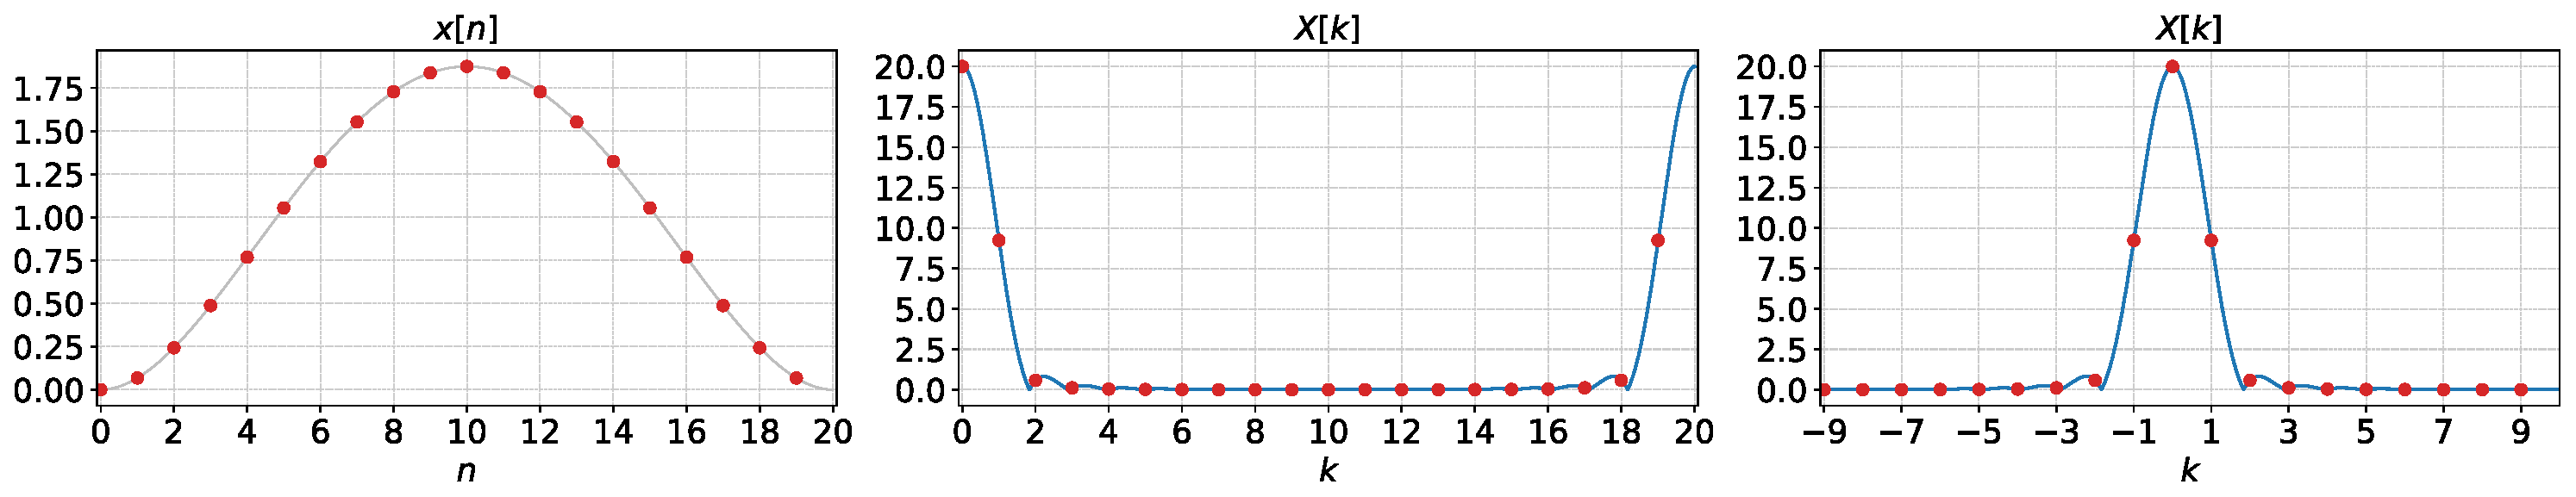
\includegraphics[width=1\textwidth]{img/dftnegfreq.eps}
  \end{figure}
\end{frame}


\begin{frame}[t]
  \frametitle{Zero-padding in the time-domain}
  Let $N$ be the length of the signal $x[n]$. The $M$-point DFT, where $M > N$ is,
  \vspace{-0.2cm}
  \[  X[k] = \sum_{n=0}^{N-1} x[n] \cdot W_M^{kn} \] 
  \vspace{-0.5cm}
  \begin{figure}
  \centering
  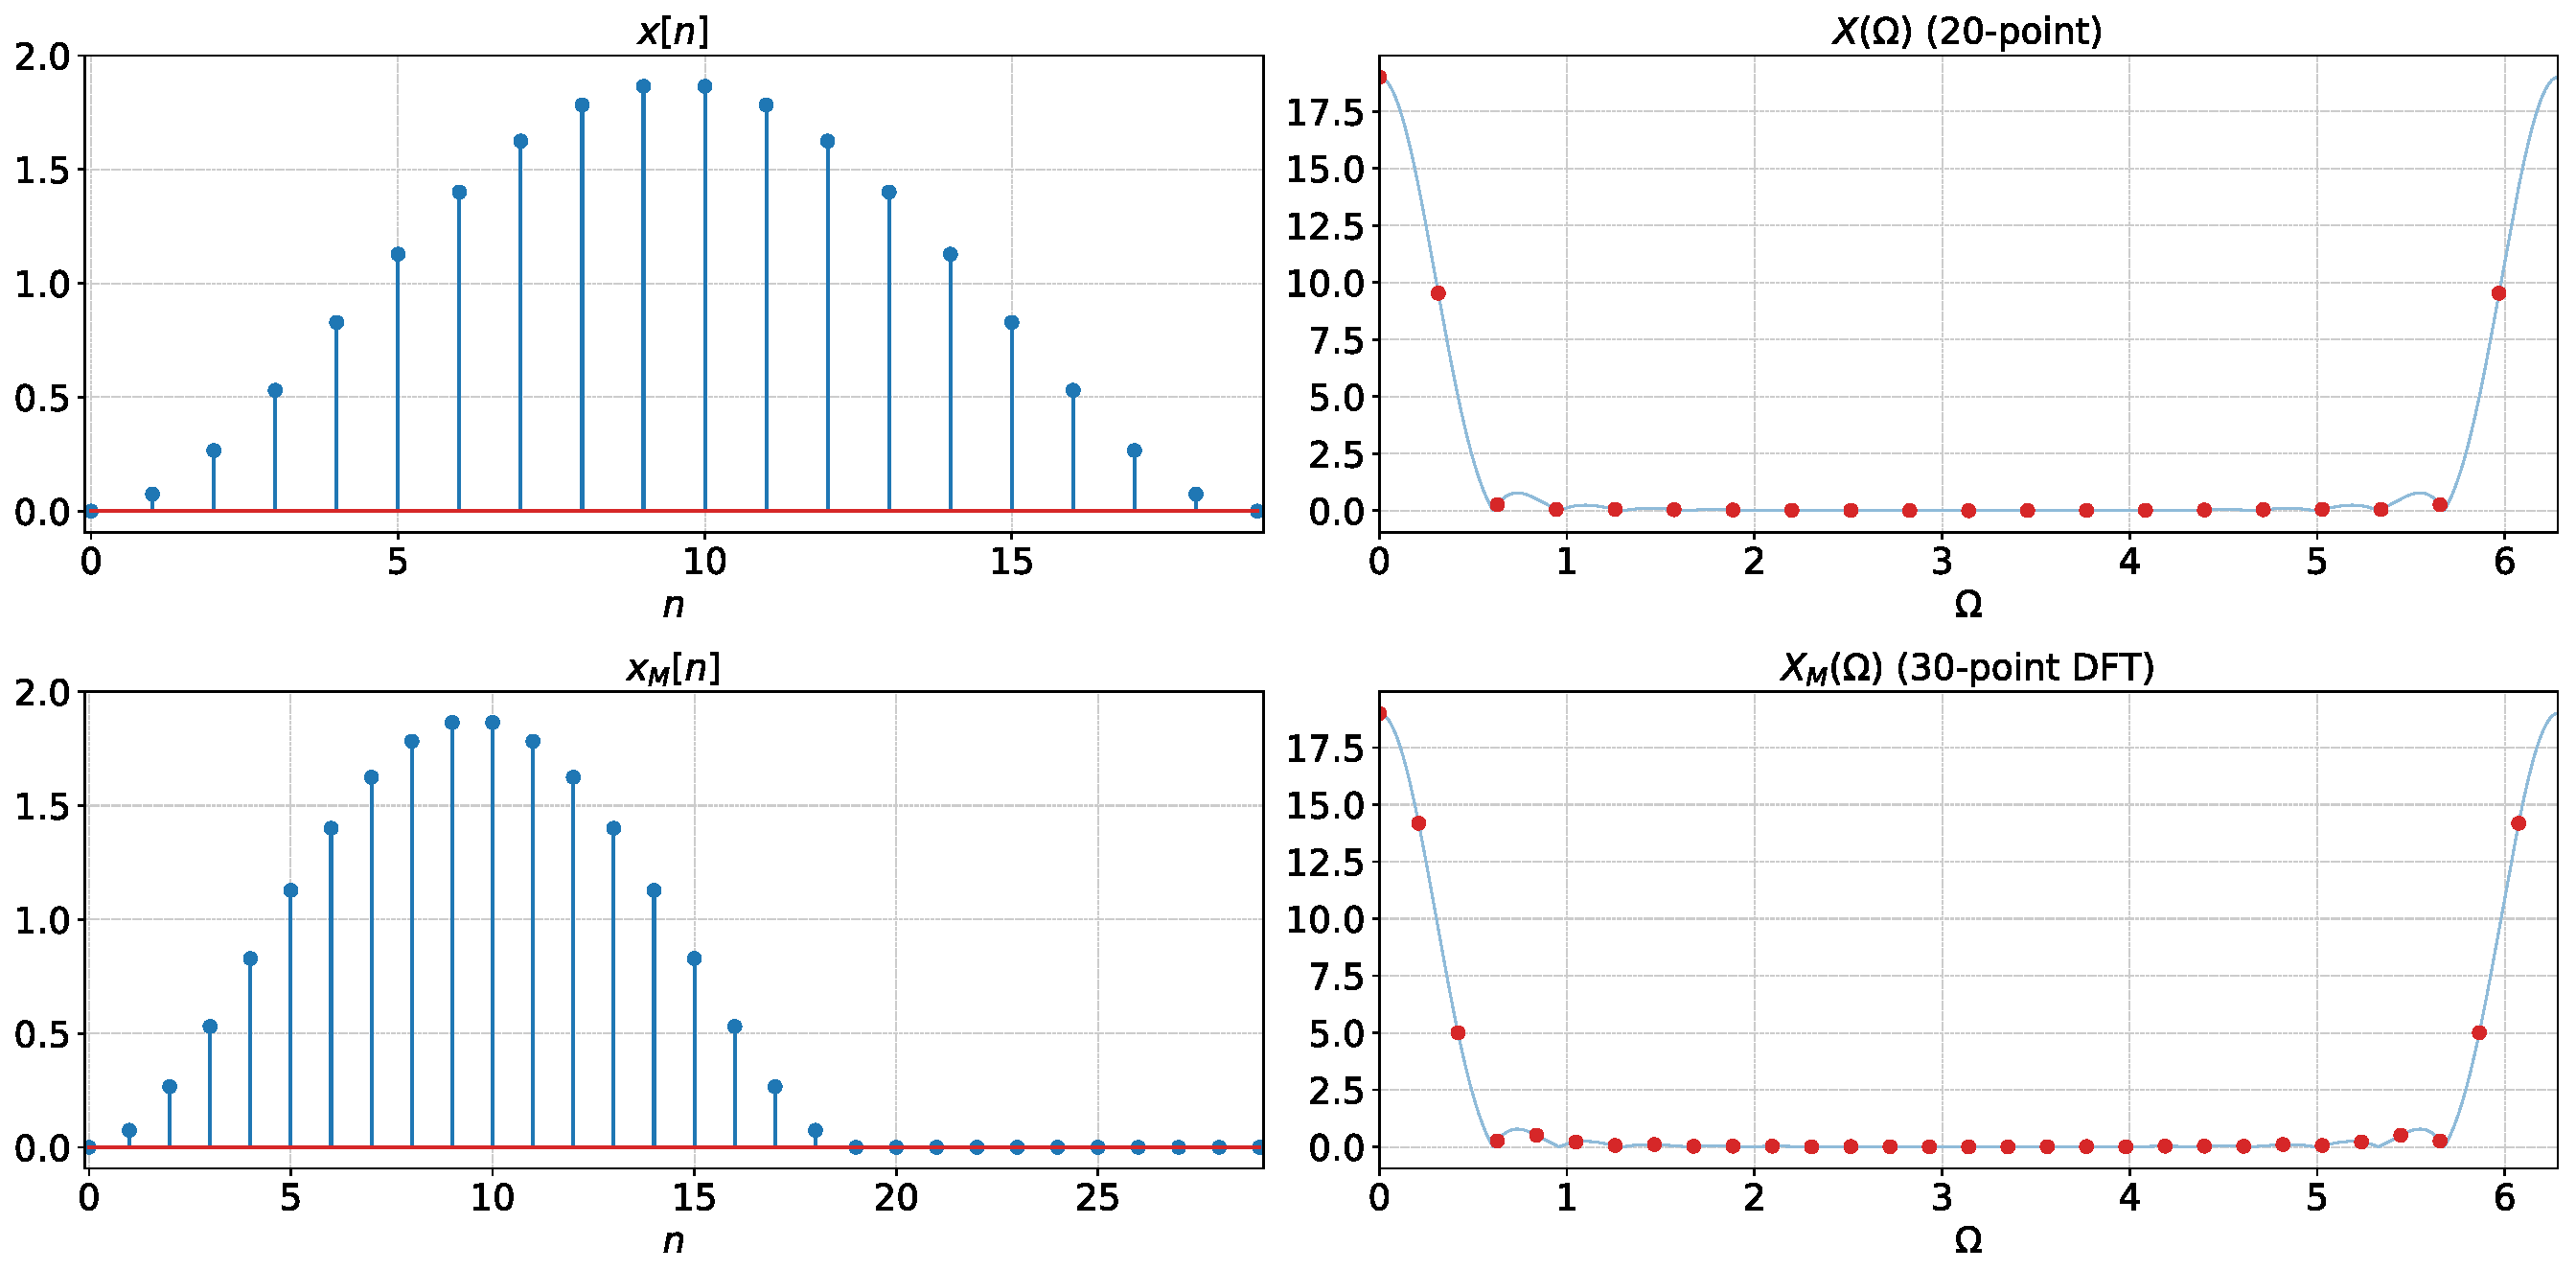
\includegraphics[width=0.8\textwidth]{img/oversampling.eps}
  \end{figure}
\end{frame}


\begin{frame}[t]
  \frametitle{Zero-padding in the time-domain}
  \begin{figure}
  \centering
  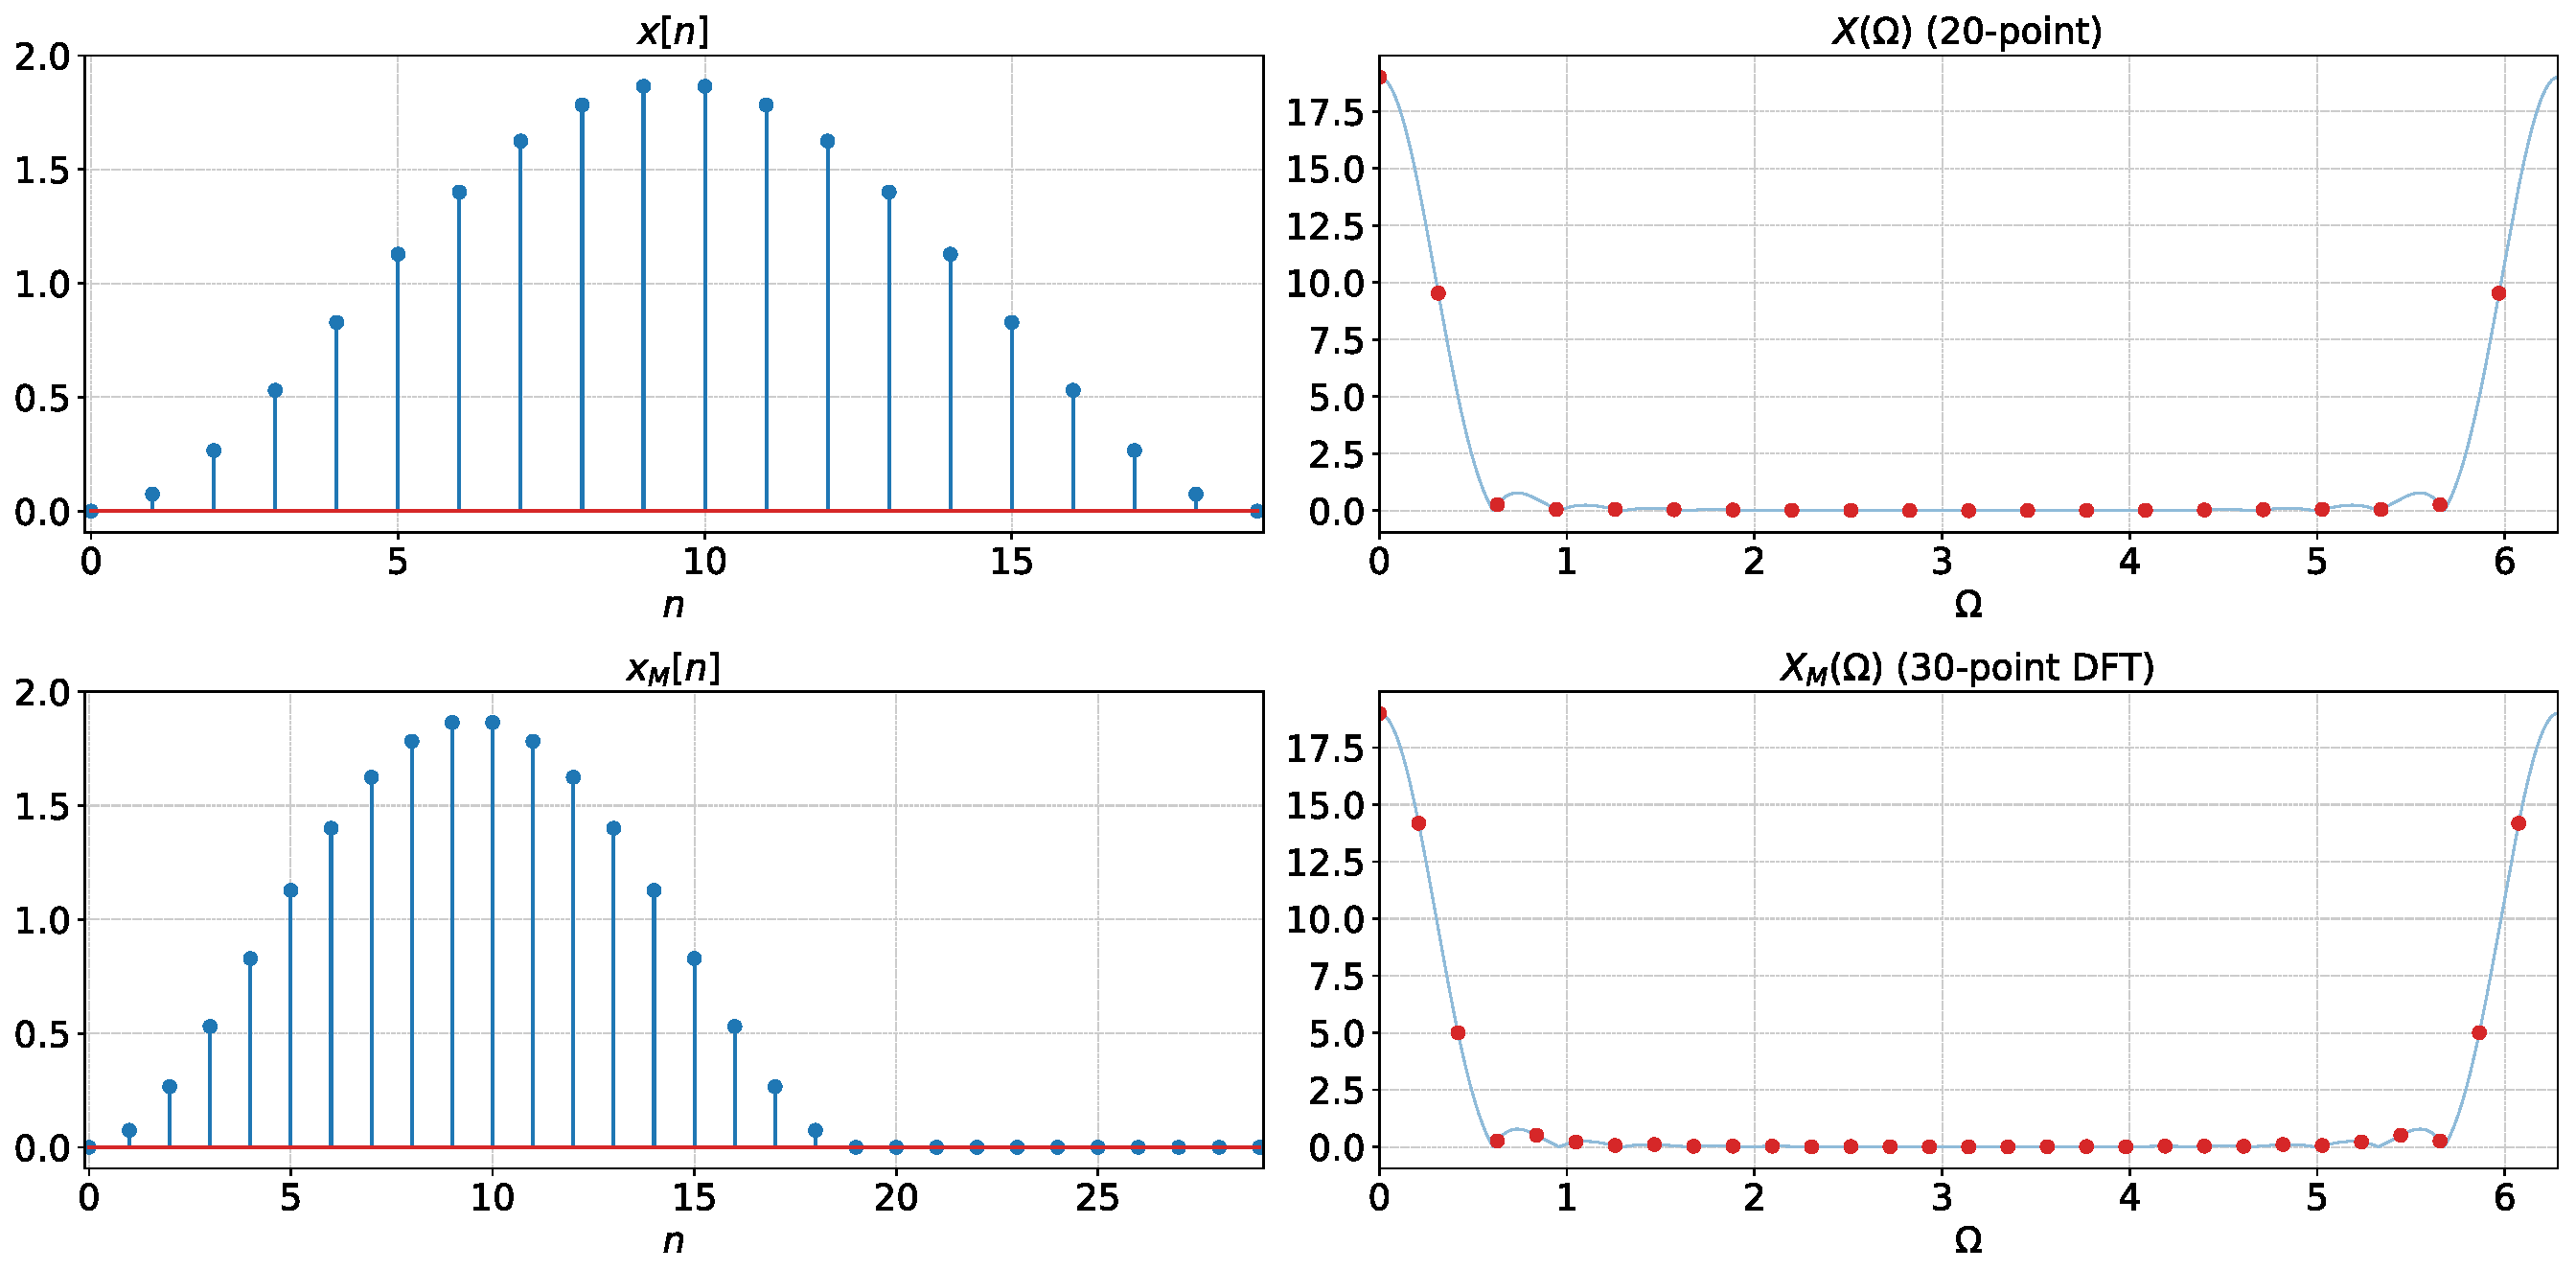
\includegraphics[width=0.6\textwidth, left]{img/oversampling.eps}
  \end{figure}
\end{frame}


\begin{frame}[t]
  \frametitle{Mapping of the $\omega$ to $\Omega$ or $k$}
  Let $x[n]$ be obtained by sampling at $F_s$ a continuous-time signal $x(t)$, whose Fourier transform is $X(\omega)$. 
  \vspace{0.25cm}

  Length of $x[n]$ is $N \,\,\, \implies \,\, x(t)$ is time-limited with duration $N\frac{1}{F_s}$.
  \vspace{0.5cm}

  \textbf{Mapping of the $\omega$ to $\Omega$ or $k$}:
  \[ \omega \in \lp -2\pi F_s, 2\pi F_s \rp \quad \mapsto \quad \Omega \in [-\pi, \pi) \quad \mapsto \quad \begin{cases} -\frac{N}{2} + 1 \leq k \leq \frac{N}{2}, & k \text{ is even} \\
  -\frac{N-1}{2} \leq k \leq \frac{N-1}{2}, & k \text{ is odd}
  \end{cases} \]

  \[ \text{Frequency corresponding to } k: \,\,\, \lp \frac{F_s}{N}\rp k \]

  \[ \text{Frequency resolution of the } N \text{-point DFT}: \,\,\, \frac{F_s}{N} \]

  You cannot increase frequency resolution by increasing sampling rate!!!!
\end{frame}


\begin{frame}[t]
  \frametitle{Zero-padding in the Frequency}
  Let $x[n]$ be obtained by sampling at $F_s$ a continuous-time signal $x(t)$, whose Fourier transform is $X(\omega)$. 
  \vspace{0.25cm}

  Length of $x[n]$ is $N \,\,\, \implies \,\, x(t)$ is time-limited with duration $N\frac{1}{F_s}$. Let's assume $N$ to be even.
  \vspace{0.25cm}

  Let $X[k]$ be the $N$-point DFT of $x[n]$, such that $-\frac{N}{2}+1 \leq k \leq \frac{N}{2}$.
  \vspace{0.25cm}

  \textbf{Zero-padding $X[k]$}: Let's append zeros to $X[k]$ to increase its length to $M$; $M$ is assumed to be even.
  \[ \tilde{X}[k] = \begin{cases}
  X[k], & -\frac{N}{2}+1 \leq k \leq \frac{N}{2} \\ 
  0, & -\frac{M}{2}+1 \leq k \leq -\frac{N}{2} \\ 
  0, & \frac{N}{2}+1 \leq k \leq \frac{M}{2} \\ 
  \end{cases} \]
\end{frame}


\begin{frame}[t]
  \frametitle{Zero-padding in the Frequency}
  \begin{figure}
  \centering
  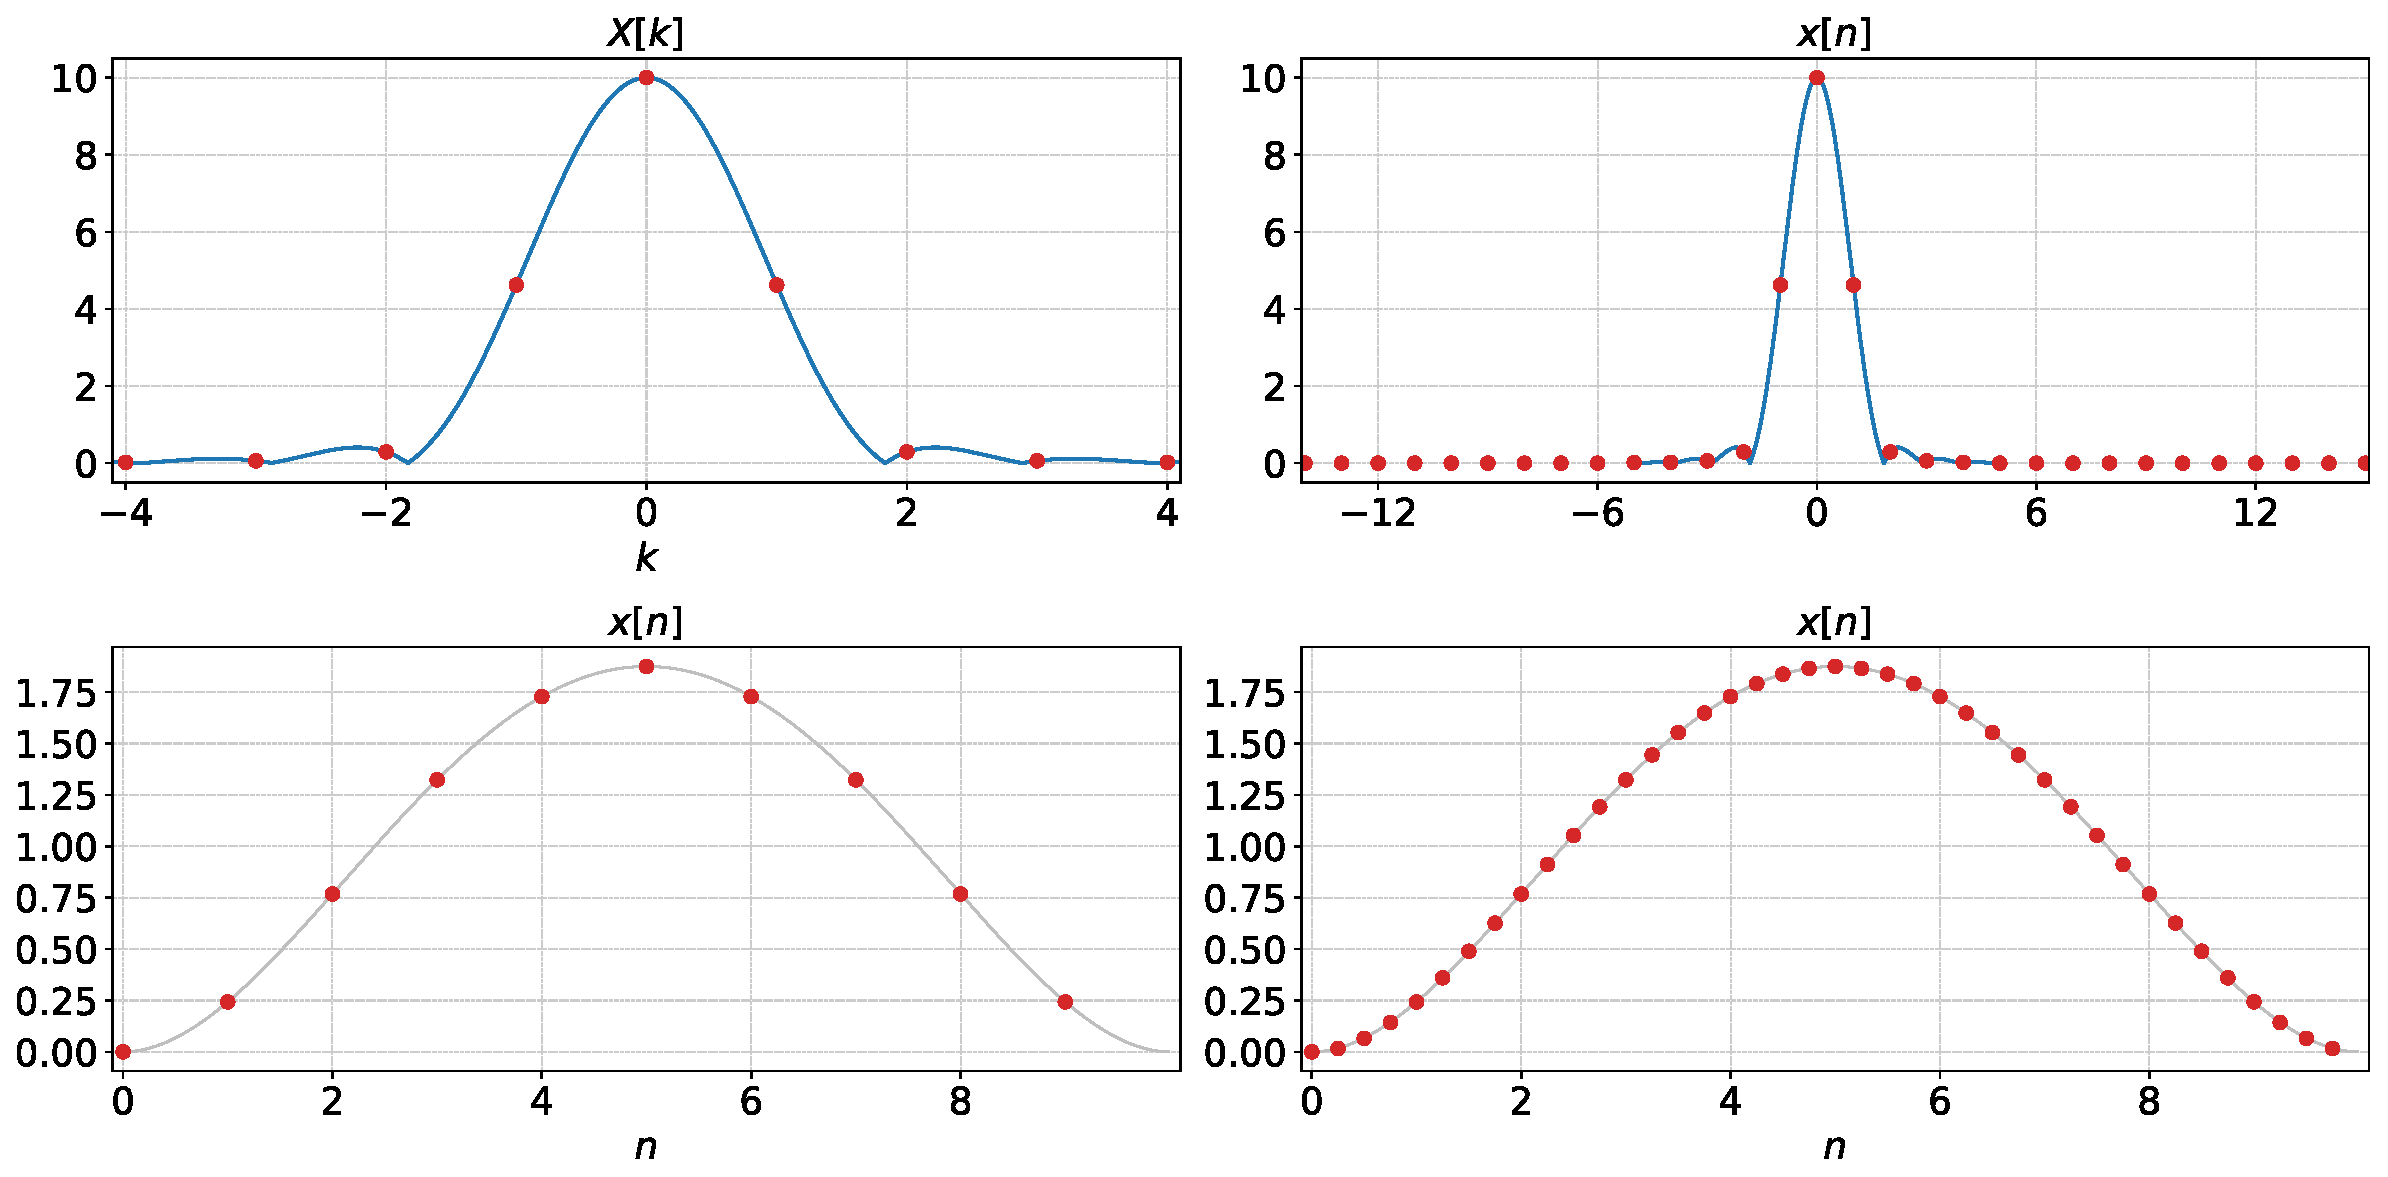
\includegraphics[width=1\textwidth]{img/oversampling-time.eps}
  \end{figure}
\end{frame}


\begin{frame}[t]
  \frametitle{Properties of DFT}
  \begin{itemize}
    \item \textbf{Periodicity}
  \end{itemize}
\end{frame}


\begin{frame}[t]
  \frametitle{Properties of DFT}
  \begin{itemize}
    \item \textbf{Symmetry of DFT}
  \end{itemize}
\end{frame}


\begin{frame}[t]
  \frametitle{Properties of DFT}
  \begin{itemize}
    \item \textbf{Multiplication and Circular Convolution}
    \[ x[n] \circledast y[n] \xleftrightarrow{\text{DFT}} X[k] \cdot Y[k] \]
  \end{itemize}
\end{frame}


\begin{frame}[t]
  \frametitle{Properties of DFT}
  \begin{itemize}
    \item \textbf{Multiplication and Circular Convolution}
    \[ x[n] \cdot y[n] \xleftrightarrow{\text{DFT}} \frac{1}{N} X[k] \circledast Y[k] \]
  \end{itemize}
\end{frame}


\begin{frame}[t]
  \frametitle{Properties of DFT}
  \begin{itemize}
    \item \textbf{Parseval's theorem}
    \[ \sum_{n=0}^{N-1} \vert x[n] \vert^2 = \frac{1}{N} \sum_{k=0}^{n-1} \vert X[k] \vert^2 \]
  \end{itemize}
\end{frame}


\begin{frame}[t]
  \frametitle{Frequency analysis of signals using DFT}
  Let $x(t)$ be a continuous-time signal of interest, and let $X\lp \omega \rp$ be its frequency spectrum.
  \[ x(t) = \cos \lp 2\pi f_0 t\rp \implies X(\omega) = \pi \delta\lp \omega + \omega_0\rp +  \pi \delta\lp \omega - \omega_0\rp  \]
  % \vspace{0.5cm}

  Sampling this signal at $F_s$Hz we get $x[n] = \cos \lp 2\pi f_0 \frac{n}{F_s}\rp = \cos \lp \frac{2\pi f_0}{F_s}n\rp$, where $\Omega_0 = \frac{2\pi f_0}{F_s}$.
  \[ X\lp \Omega \rp = \pi \delta\lp \Omega + \Omega_0\rp + \pi \delta\lp \Omega - \Omega_0 \rp \]

  In practice, we only take a finite number of samples from $x[n]$ for analysis. Let the number of samples be $N$, and thus the duration of the signal considered for analysis if $T = \frac{N}{F_s}$.

  \[ x_a[n] = \begin{cases} x[n], & 0 \leq n < N \\ 0, & \text{Otherwise} \end{cases} = x[n] \cdot w[n] \]

  where, $w[n] = \begin{cases} 1, & 0 \leq n < N \\ 0, & \text{Otherwise} \end{cases}$.
\end{frame}


\begin{frame}[t]
  \frametitle{Frequency analysis of signals using DFT}
  \begin{figure}
  \centering
  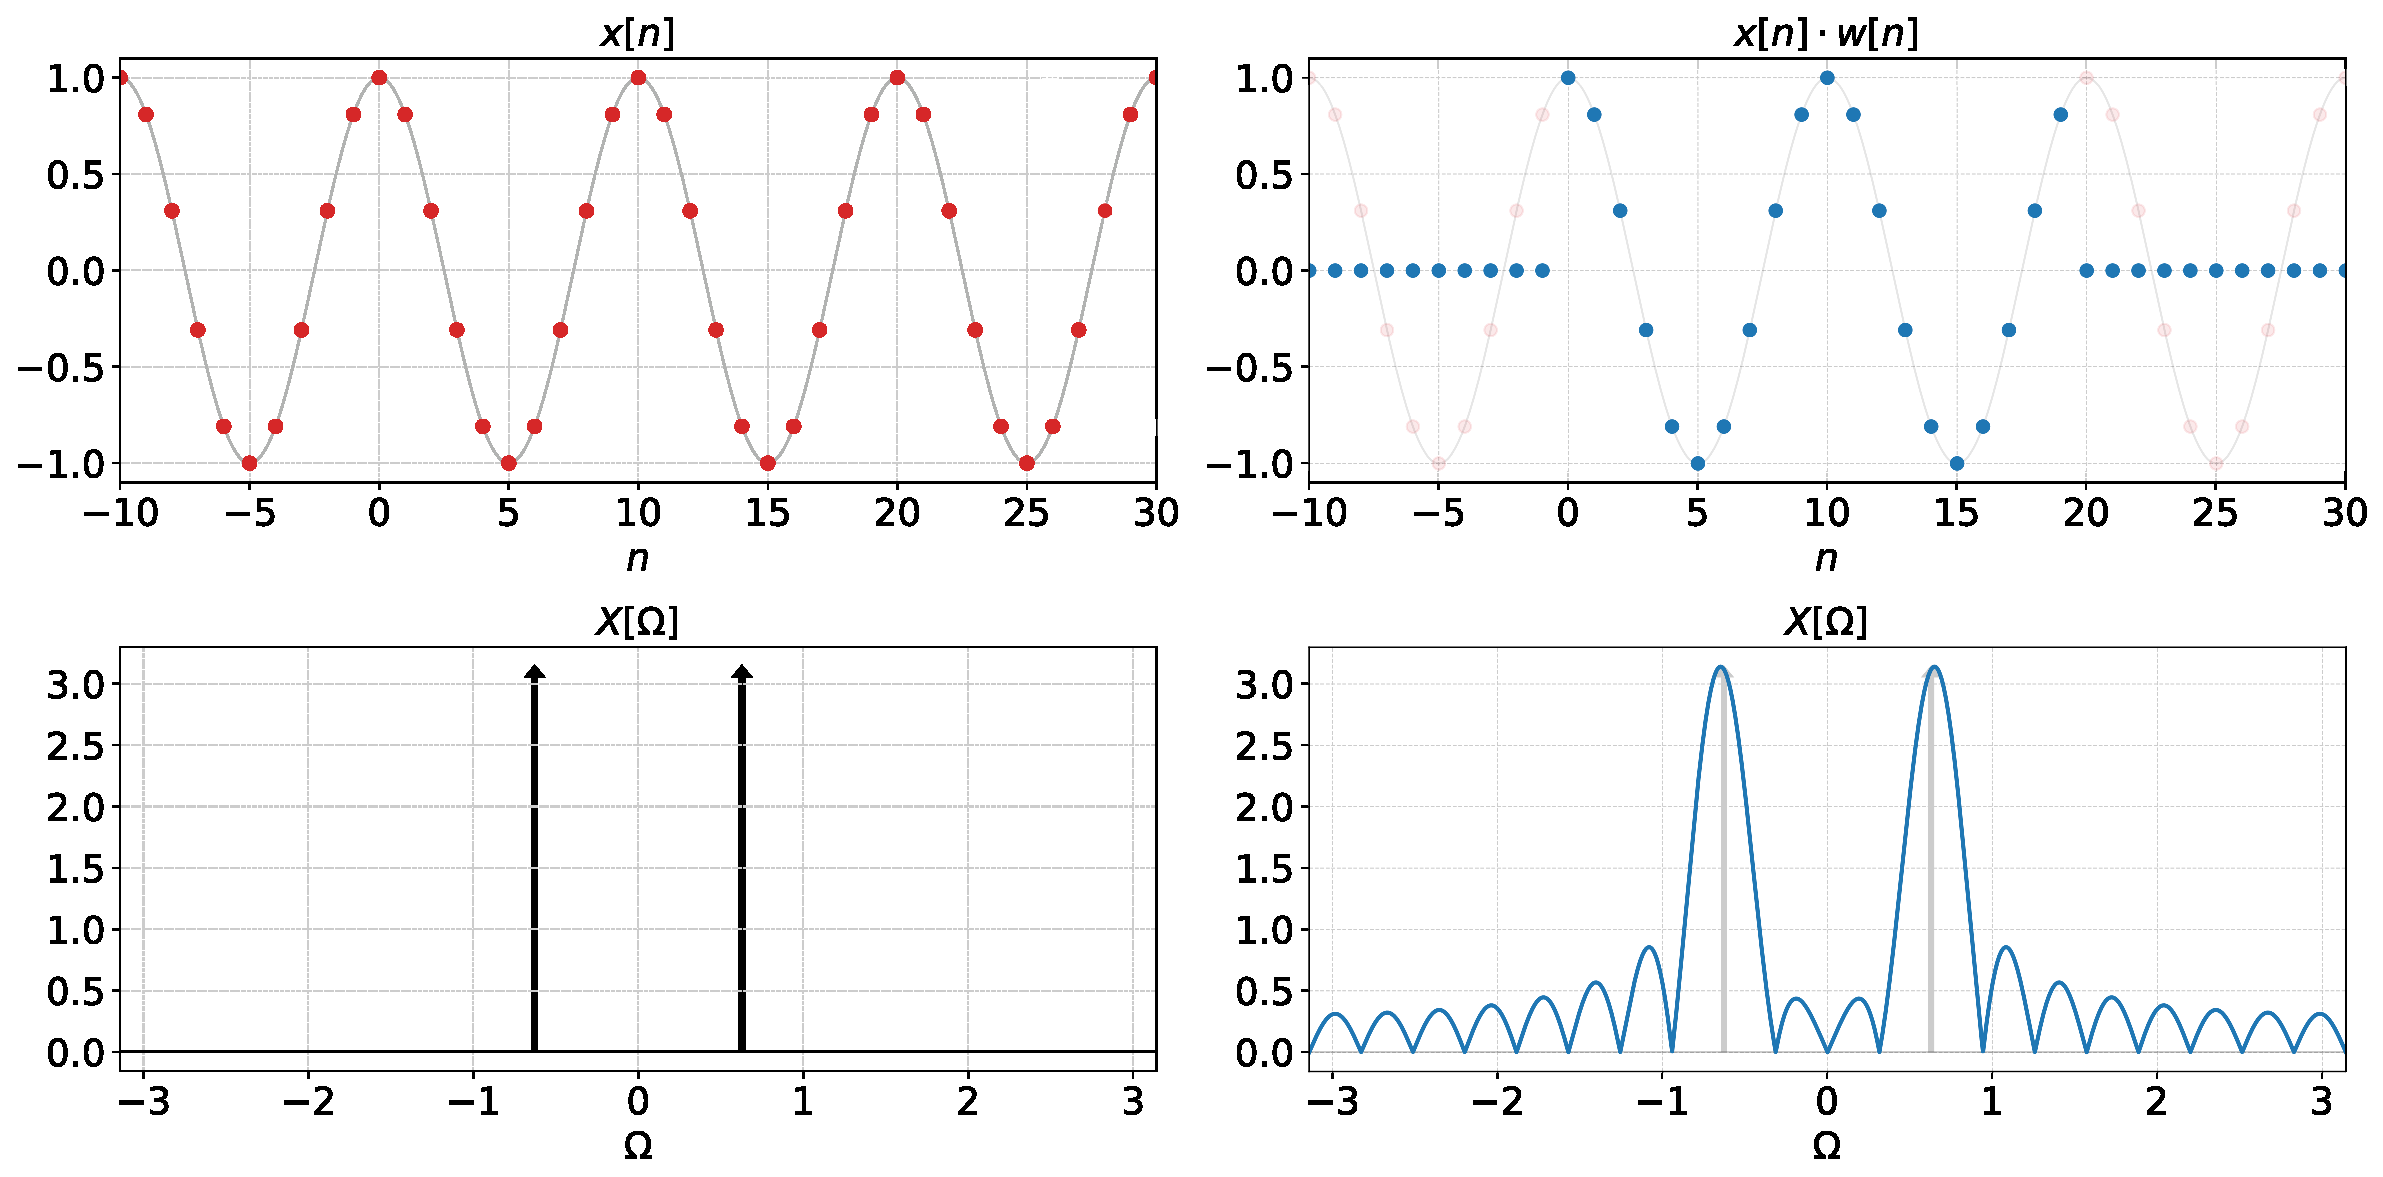
\includegraphics[width=1\textwidth]{img/dft-leakage.eps}
  \end{figure}
\end{frame}


\begin{frame}[t]
  \frametitle{Frequency analysis of signals using DFT}
  \begin{figure}
  \centering
  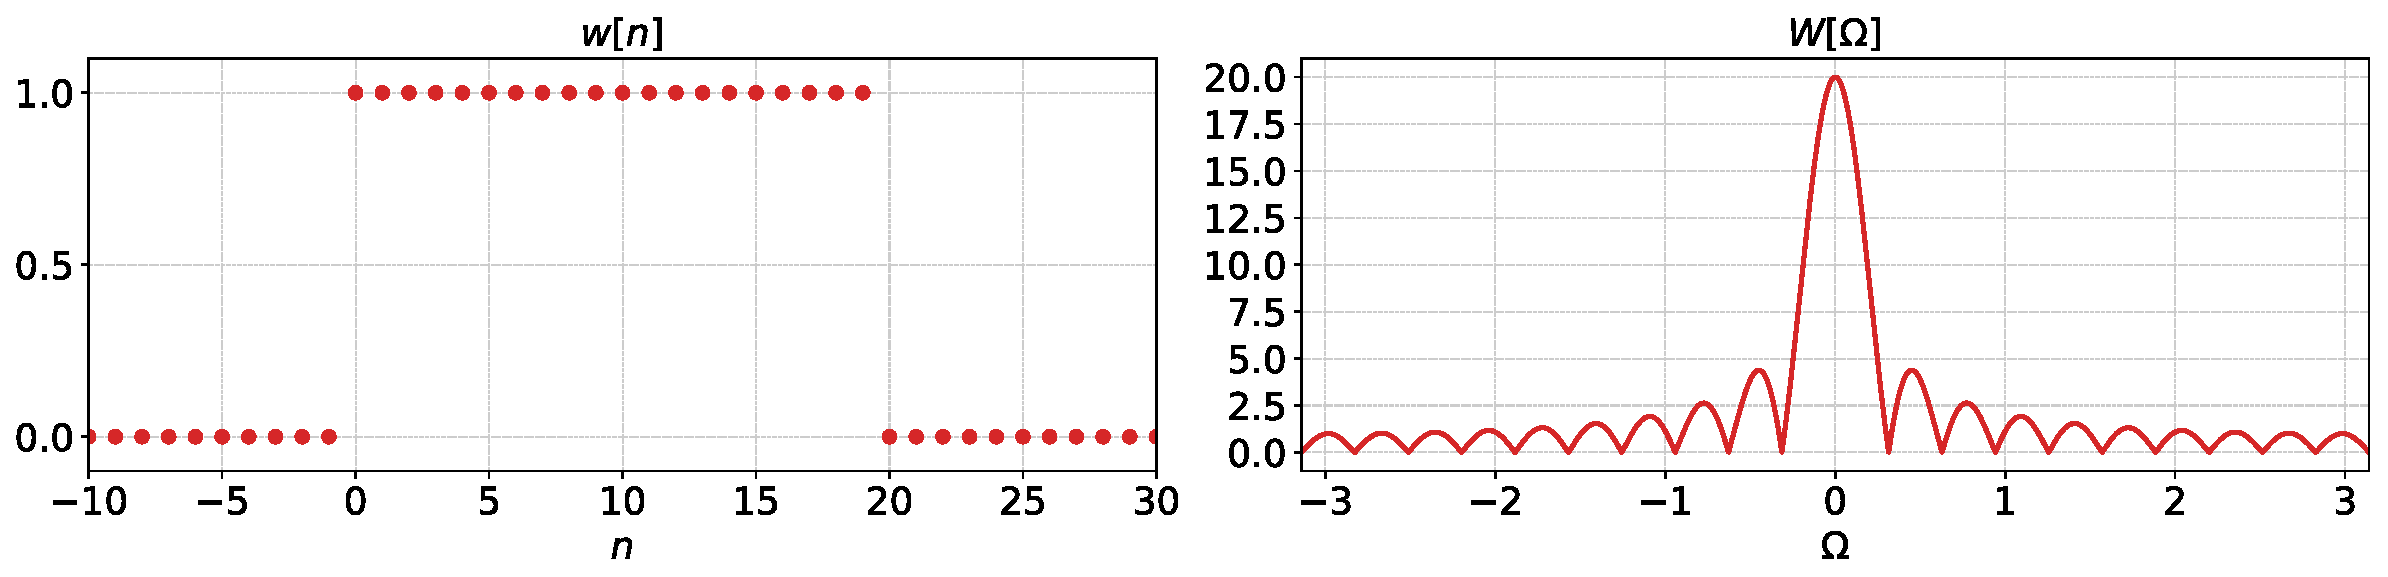
\includegraphics[width=1\textwidth, left]{img/dft-rectwindow.eps}
  \end{figure}

  \[ W\lp \Omega \rp = \frac{\sin \lp \Omega N / 2\rp}{\sin \lp \Omega / 2\rp}e^{-j \Omega \lp N - 1\rp / 2} \]
\end{frame}


\begin{frame}[t]
  \frametitle{Frequency analysis of signals using DFT}
  \begin{figure}
  \centering
  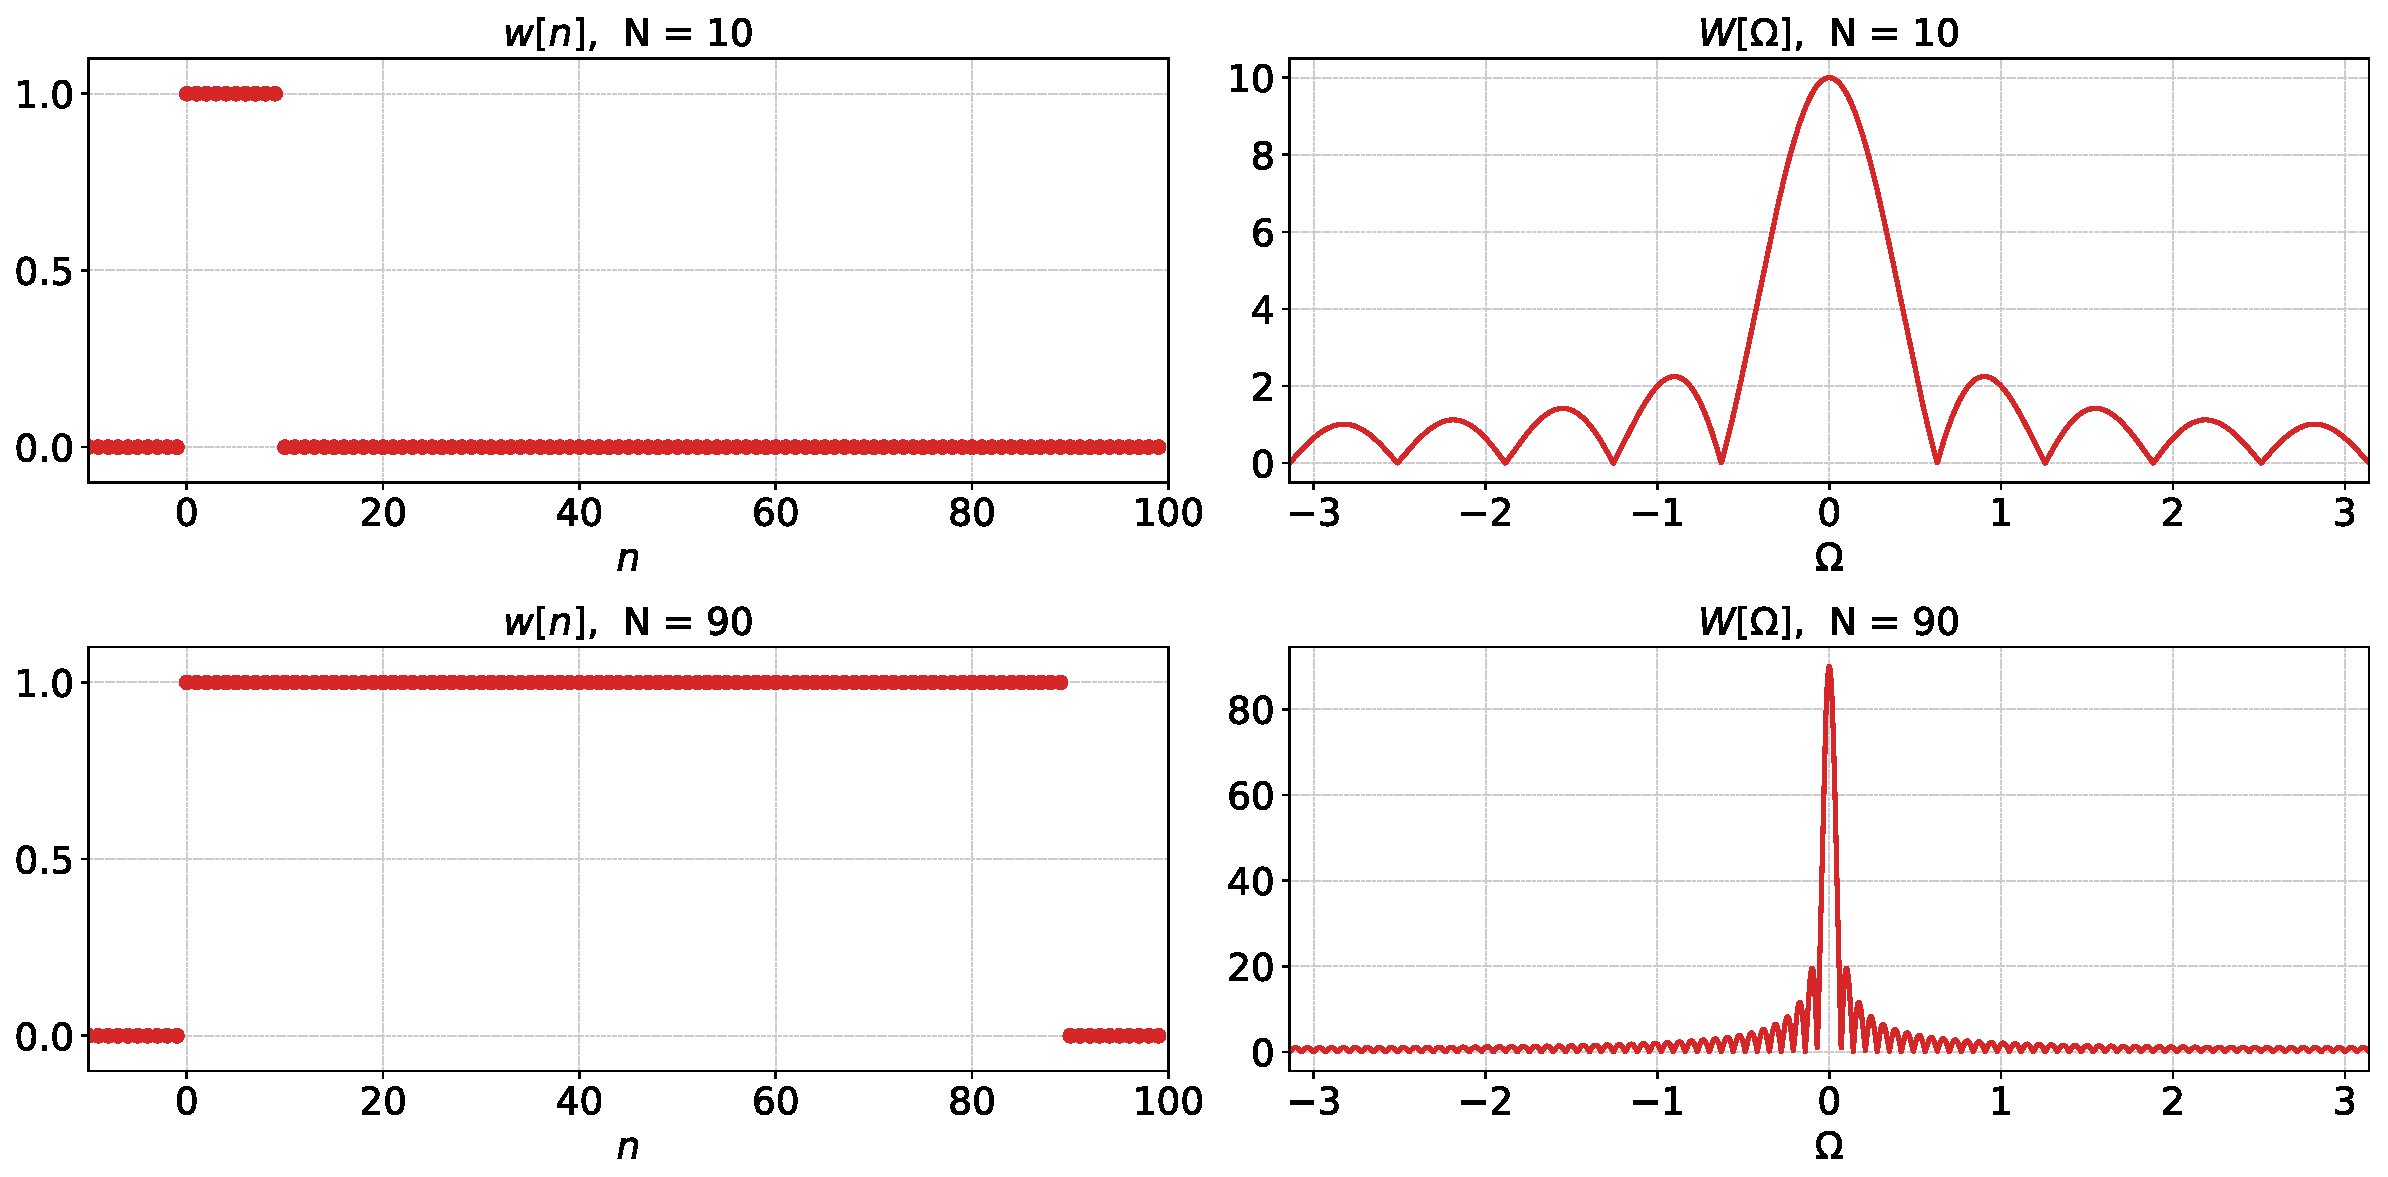
\includegraphics[width=1\textwidth, left]{img/dft-rectwindows.eps}
  \end{figure}
\end{frame}


\begin{frame}[t]
  \frametitle{Frequency analysis of signals using DFT}
  Consider the signal $x(t)$ sampled at $F_s = 10Hz$.
  \[ x(t) = \cos \lp 2\pi t \rp + \cos\lp 4 \pi t\rp \]
  \begin{figure}
  \centering
  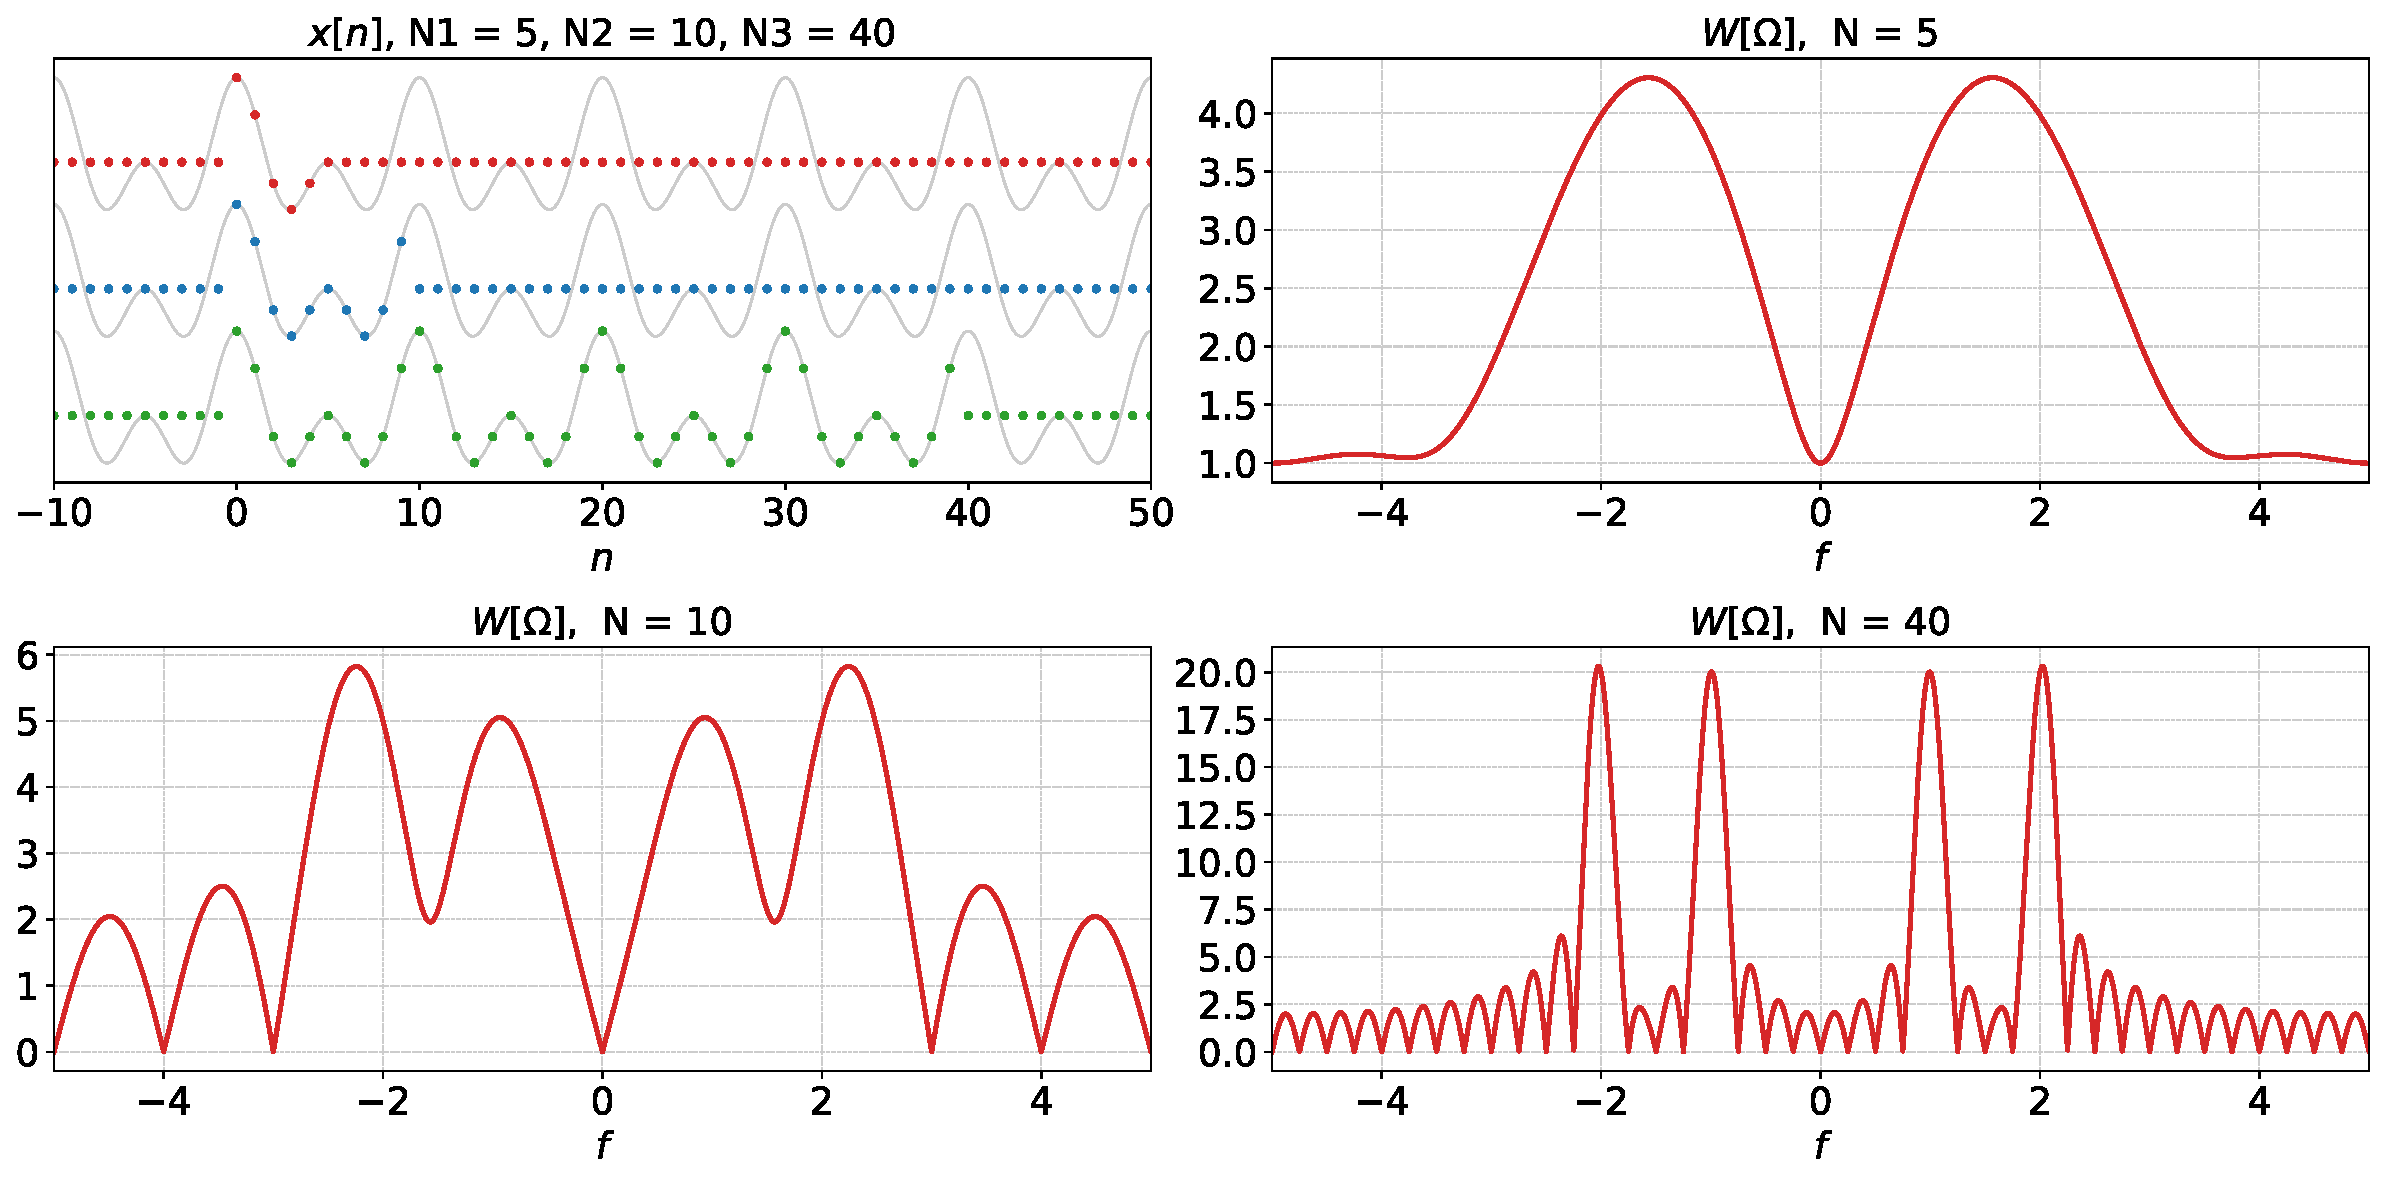
\includegraphics[width=0.82\textwidth]{img/dft-resolve1.eps}
  \end{figure}
\end{frame}


\begin{frame}[t]
  \frametitle{Frequency analysis of signals using DFT}
  Resolving two frequencies depends on the size of the rectangular window.
  \[ W\lp \Omega \rp = \frac{\sin \lp \Omega N / 2\rp}{\sin \lp \Omega / 2\rp}e^{-j \Omega \lp N - 1\rp / 2} \]

  Condition on the window size for resolving signals with close frequencies,
  \[ \vert \Omega_1 - \Omega_2 \vert \geq \frac{2\pi}{N} \]

  When data is sampled at $F_s$, then
  \[ \vert f_1 - f_2 \vert \geq \frac{F_s}{N} \]
\end{frame}


\begin{frame}[t]
  \frametitle{Frequency analysis of signals using DFT}
  Consider the signal $x(t)$ sampled at $F_s = 10Hz$.
  \[ x(t) = \cos \lp 2\pi t \rp + 0.5\cos\lp 4 \pi t\rp \]
  \begin{figure}
  \centering
  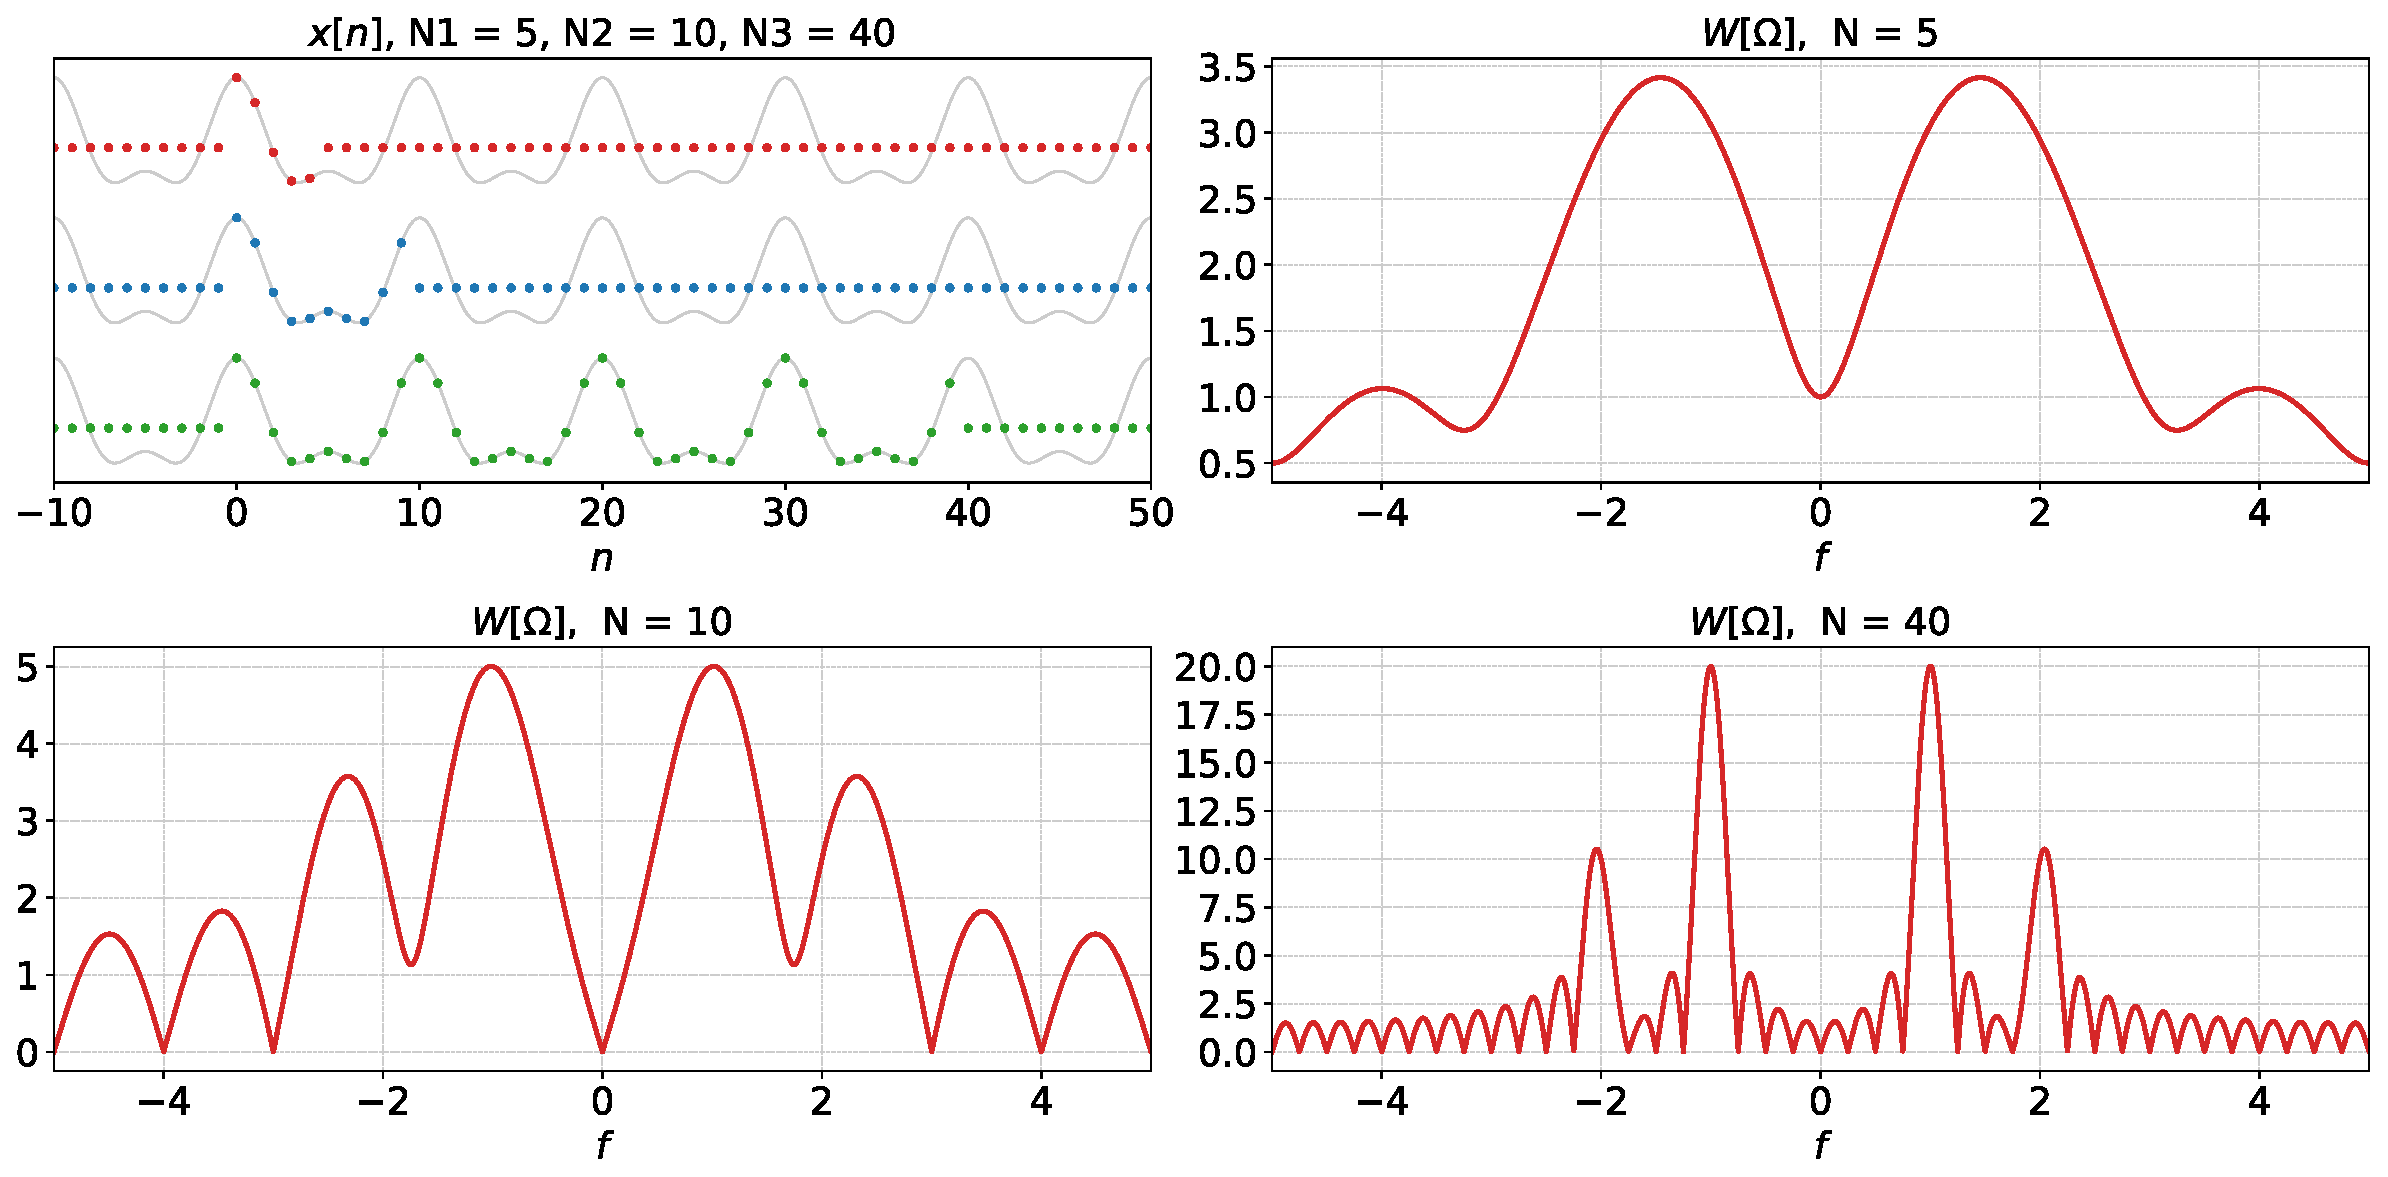
\includegraphics[width=0.82\textwidth]{img/dft-resolve2.eps}
  \end{figure}
\end{frame}


\begin{frame}[t]
  \frametitle{Other windows for DFT analysis}
  \begin{figure}
  \centering
  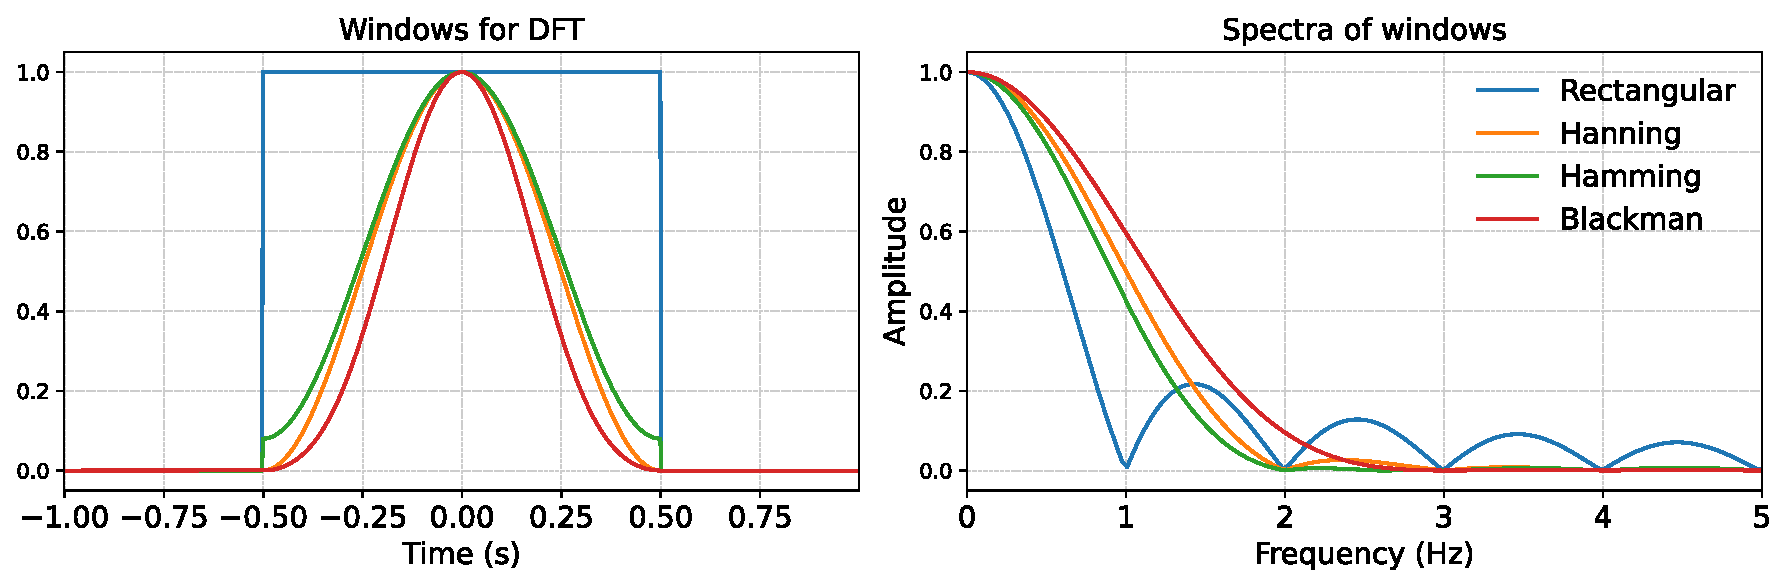
\includegraphics[width=1\textwidth]{img/dft-windows.eps}
  \end{figure}
\end{frame}


\begin{frame}[t]
  \frametitle{Frequency analysis of signals using DFT: Hamming Window}
  \begin{figure}
  \centering
  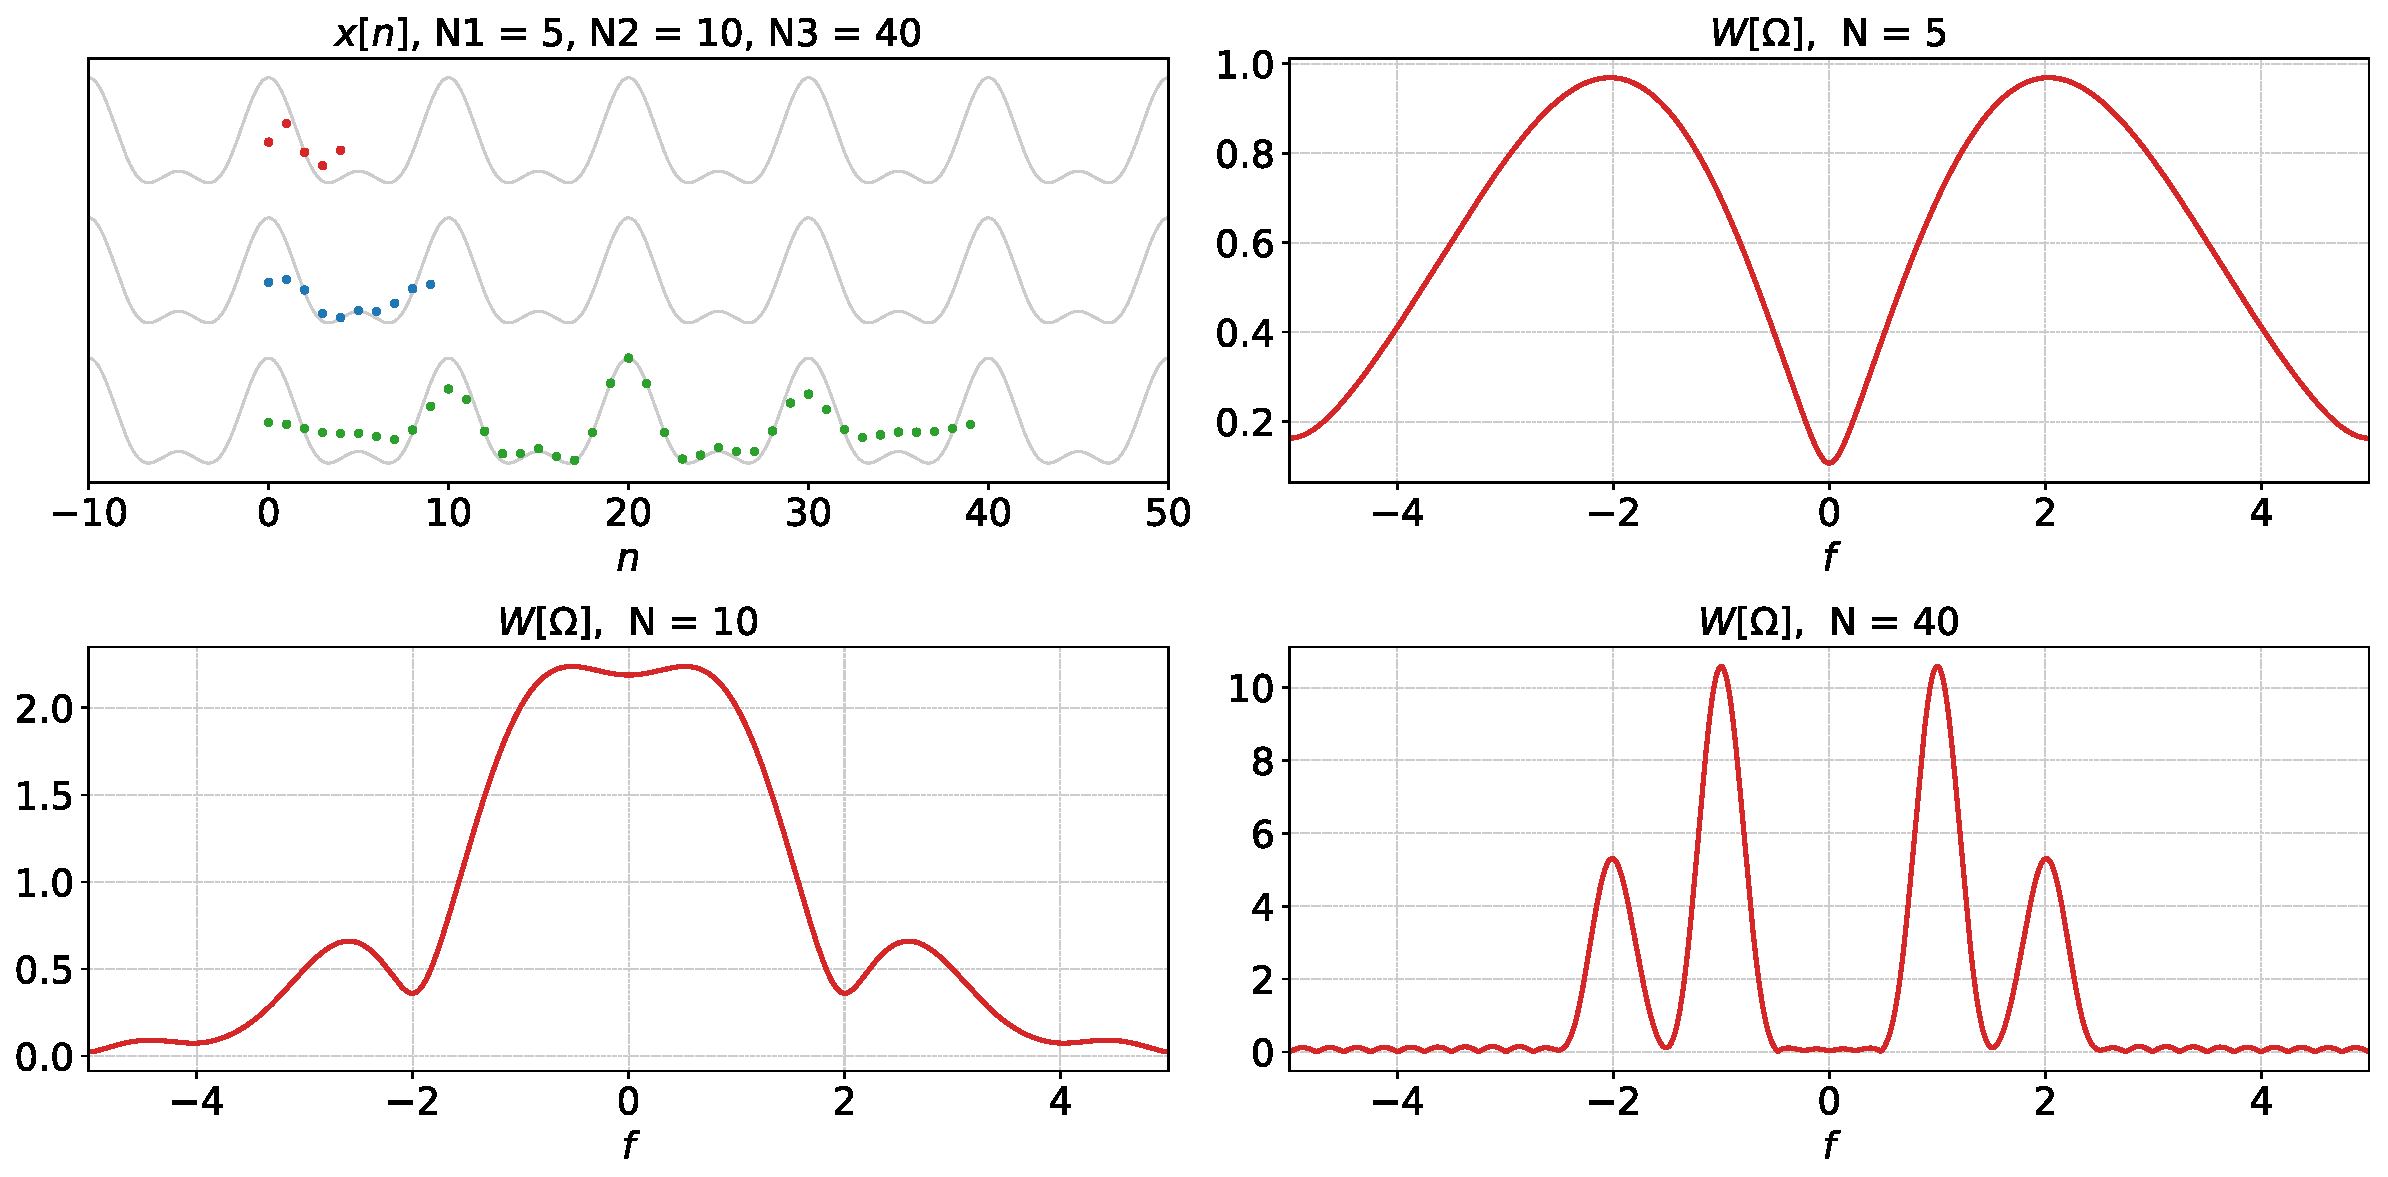
\includegraphics[width=1\textwidth]{img/dft-resolve2-hamming.eps}
  \end{figure}
\end{frame}


\begin{frame}[t]
  \frametitle{Frequency analysis of signals using DFT: Hamming Window}
  \begin{figure}
  \centering
  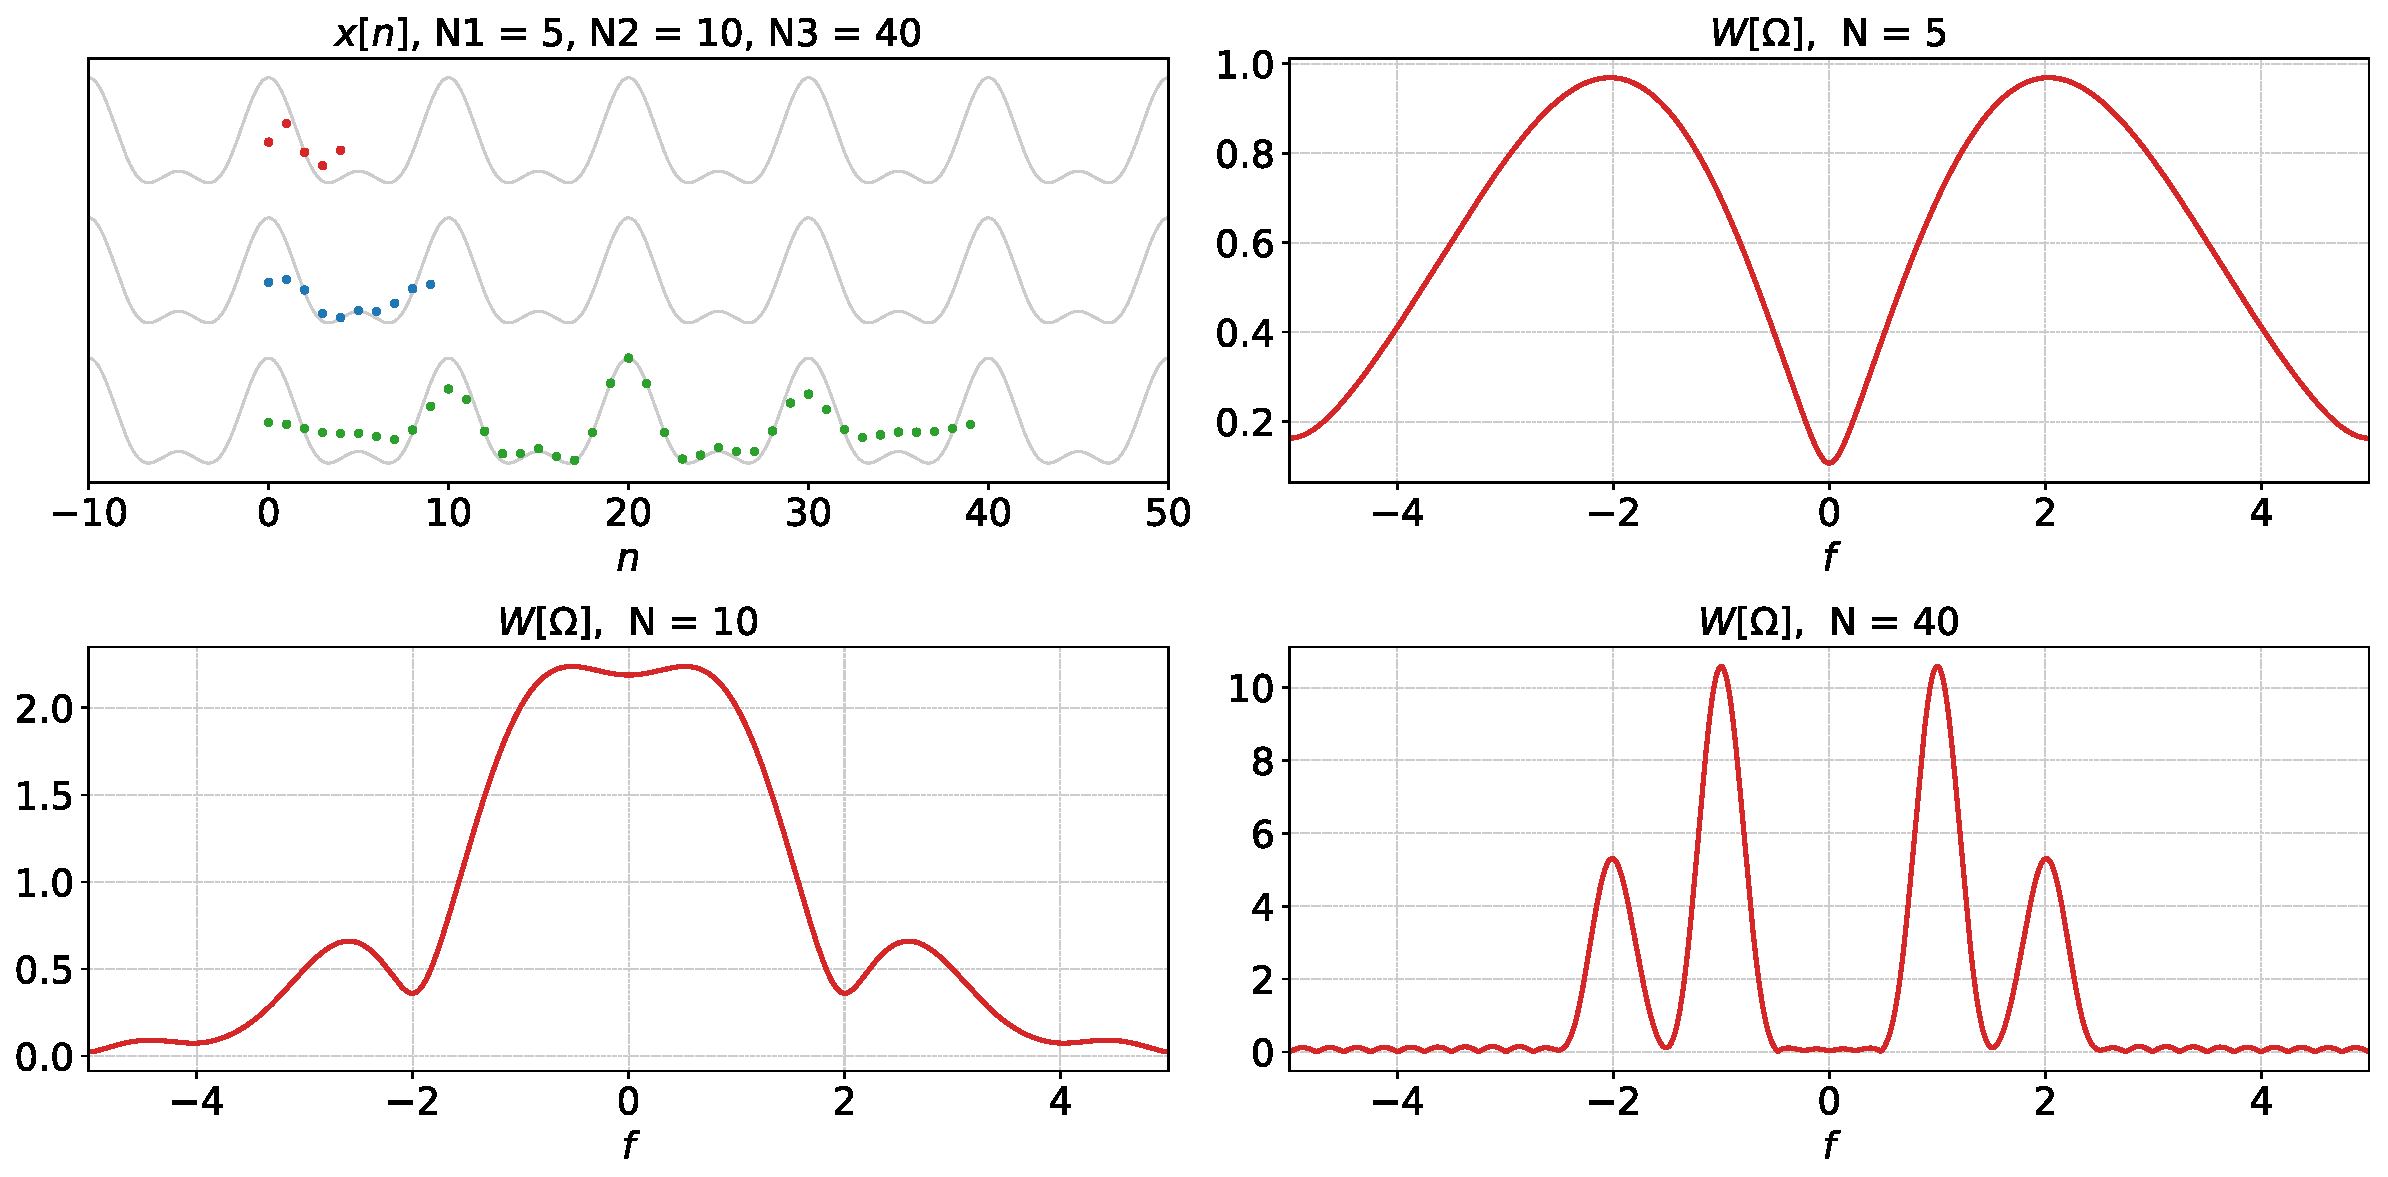
\includegraphics[width=1\textwidth]{img/dft-resolve2-hamming.eps}
  \end{figure}
\end{frame}


\begin{frame}[t]
  \frametitle{Another effect of window length}
  \begin{figure}
  \centering
  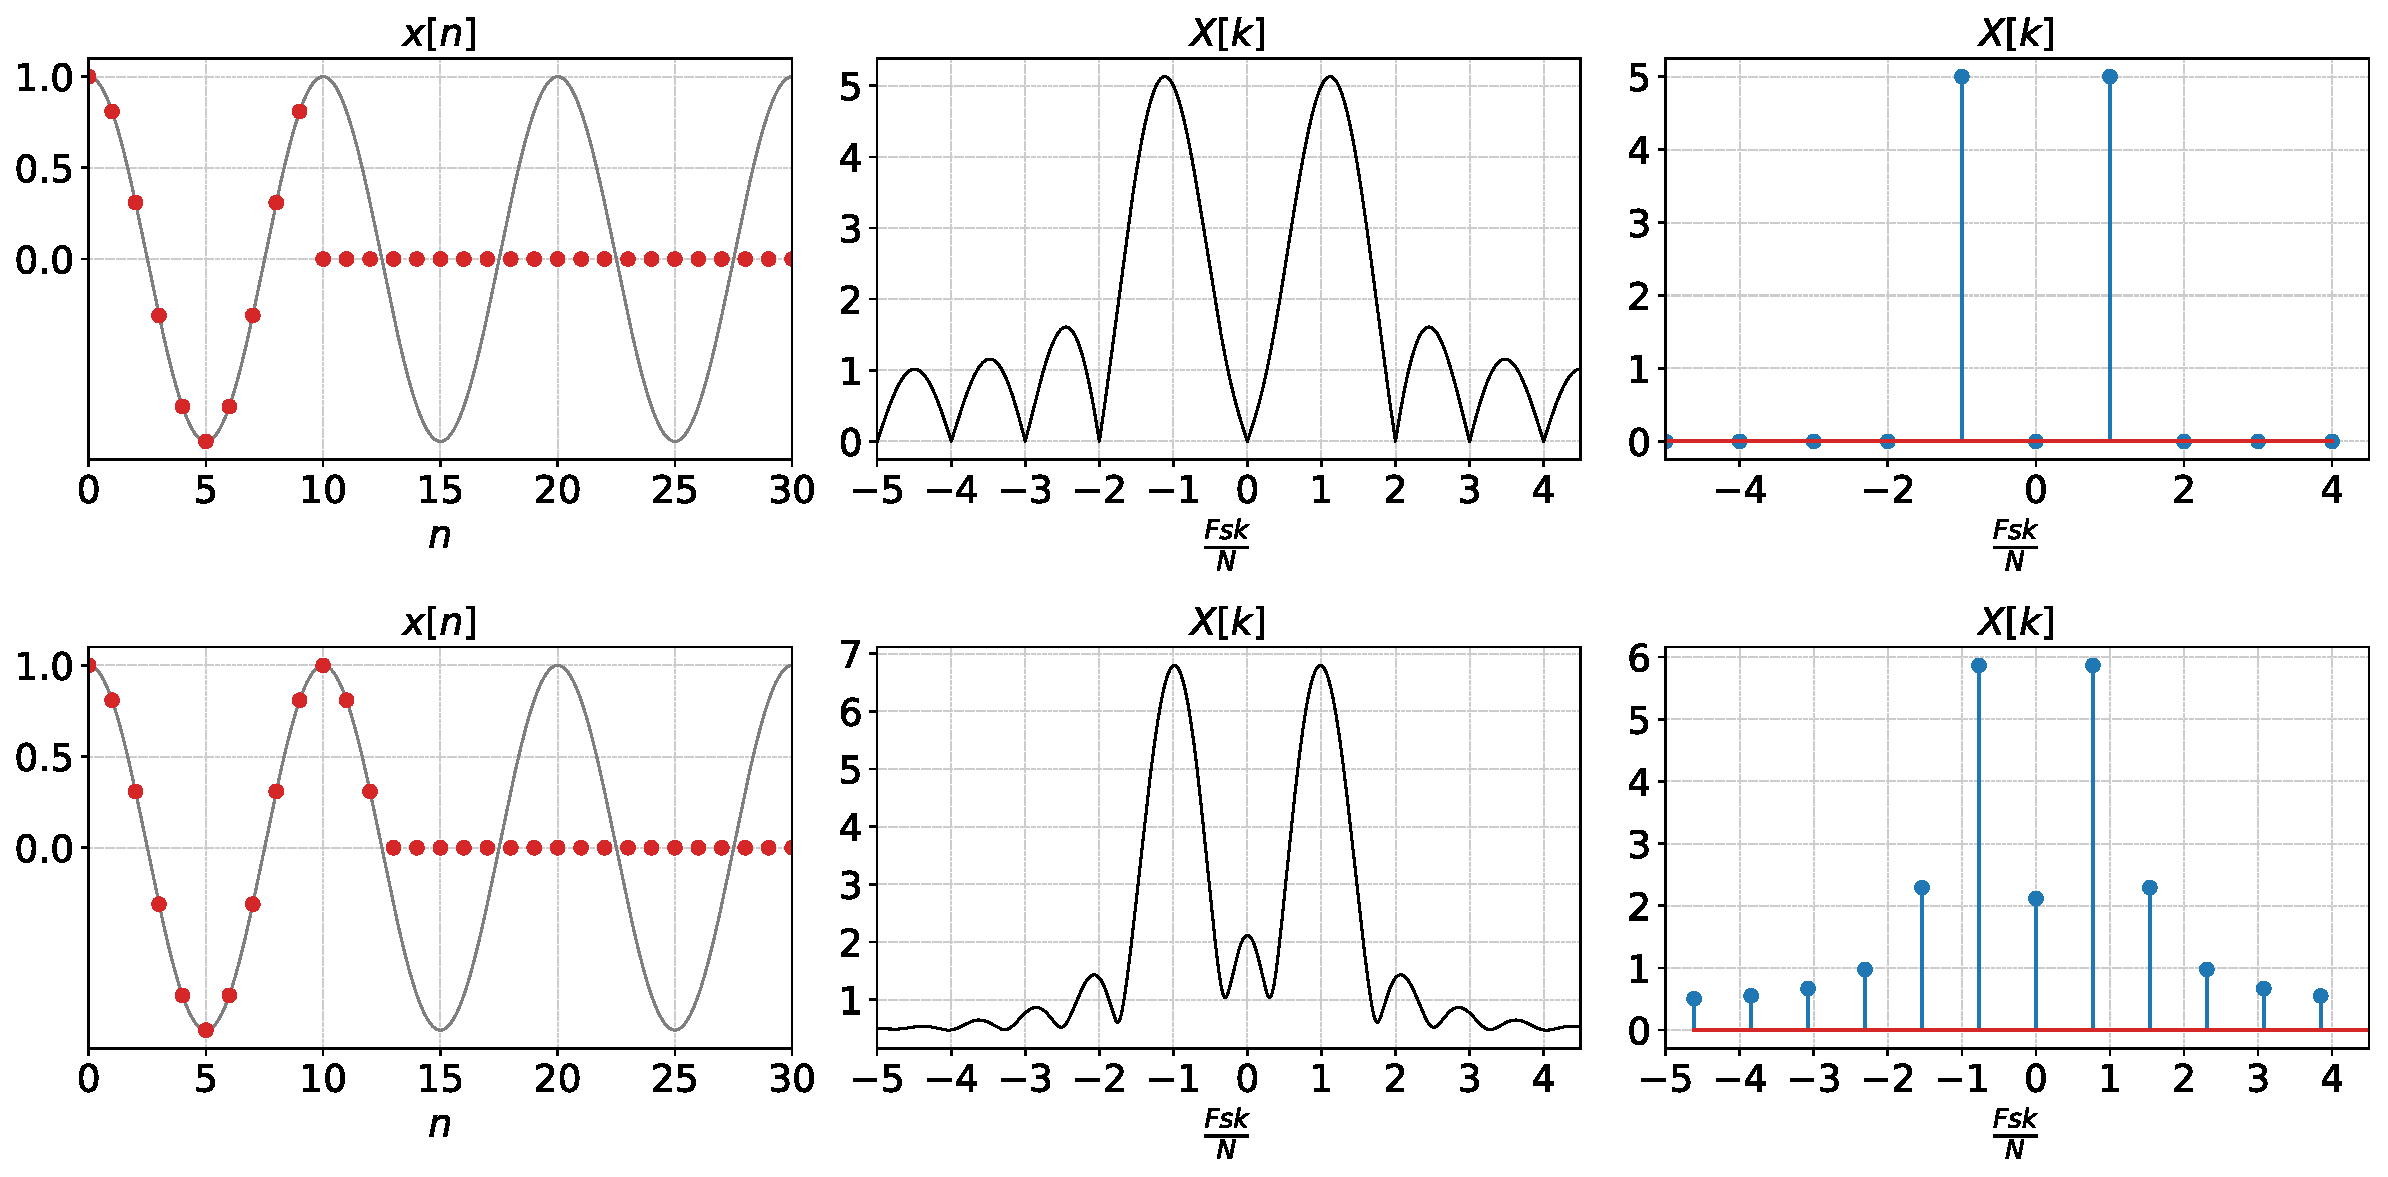
\includegraphics[width=1\textwidth]{img/dft-windoweffect.eps}
  \end{figure}
\end{frame}



% \begin{frame}[t]{Response of an LTI system to a complex exponential}
% \[ H(\Omega) = \sum_{k=-\infty}^{\infty} h[k]e^{-j\Omega k} = \big \vert H\lp \Omega \rp \big \vert e^{j \Theta\lp \Omega \rp}  \]

% where, 
% \begin{itemize}
%   \item $\vert H\lp \Omega \rp \vert$ is the mangitude response.
%   \item $\Theta\lp \Omega \rp = \arg \{ H\lp \Omega \rp \}$ is the phase response.
% \end{itemize}
% \vspace{1cm}

% The output to $A e^{j\Omega n}$ is given by,
% \[ A e^{j \Omega n} \longrightarrow A \big \vert H \lp \Omega \rp\big \vert e^{j \{ \Omega n + \Theta\lp \Omega\rp\}} \]

% \end{frame}


% \begin{frame}[t]{Response of an LTI system to a complex exponential}
% \textbf{Moving average filter}
% \[ y[n] = \frac{1}{3} \lp x[n+1] + x[n] + x[n-1] \rp \]

% \end{frame}


% \begin{frame}[t]{Response of an LTI system to a complex exponential}
%   \begin{center}
%   \begin{figure}
%   \centering
%   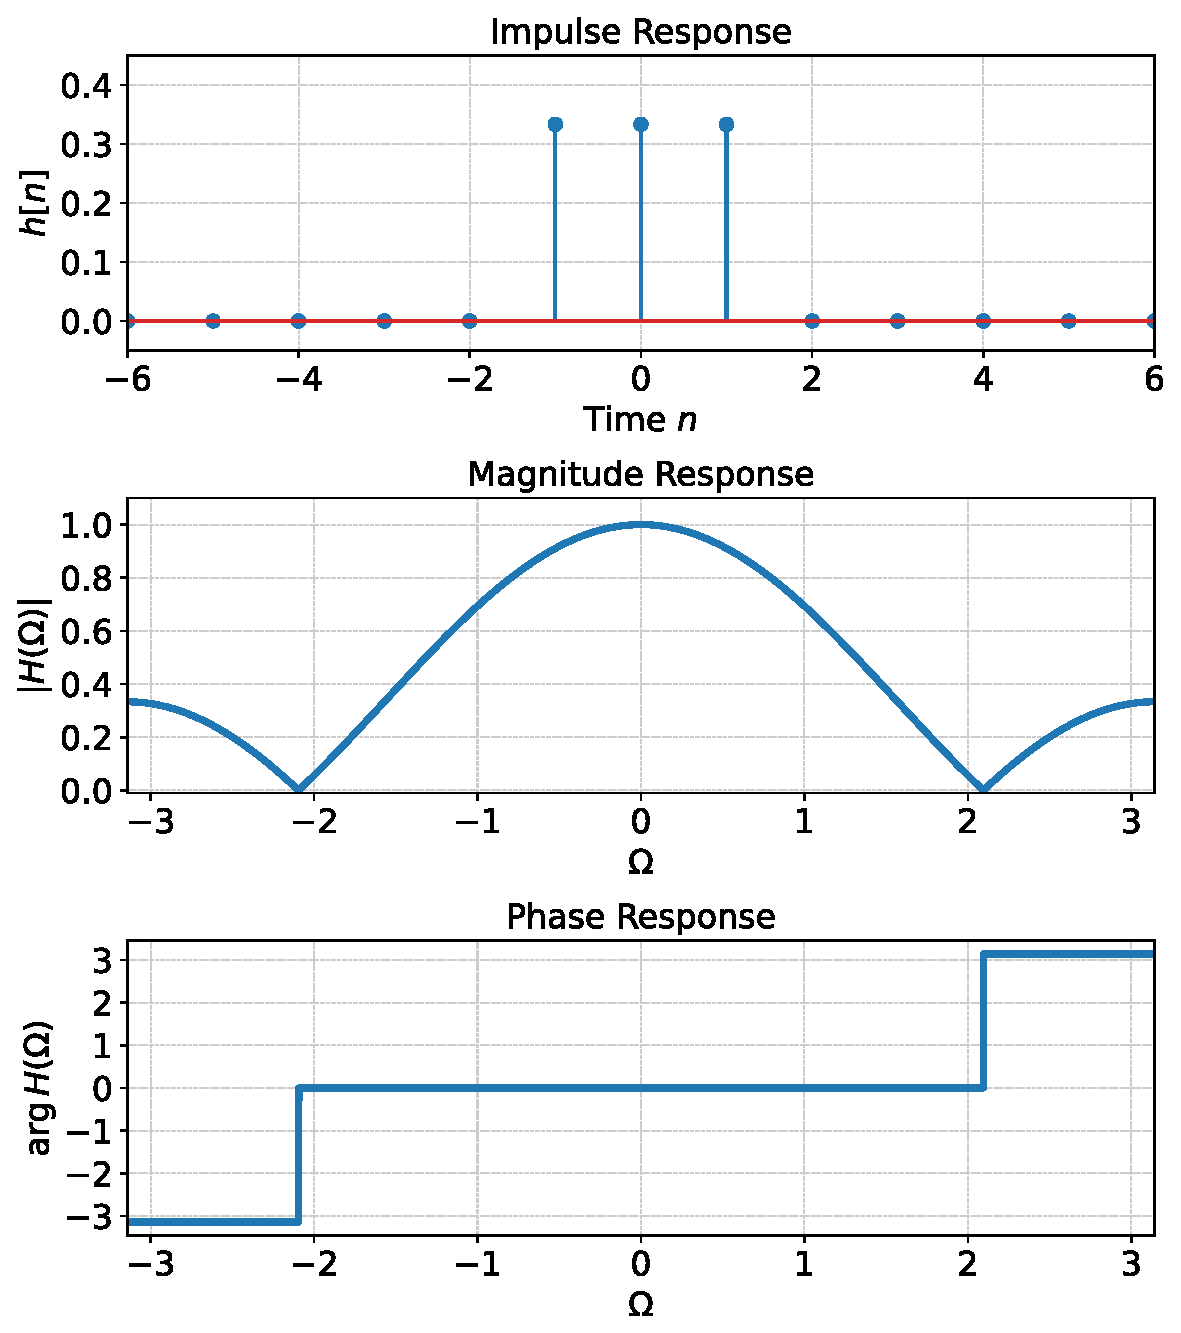
\includegraphics[width=0.4\textwidth]{img/movavg.eps}
%   \end{figure}
%   \end{center}
% \end{frame}


% \begin{frame}[t]{Response of an LTI system to a complex exponential}
% \[ x[n] \rightarrow X\lp \Omega \rp \longrightarrow H\lp \Omega \rp X\lp \Omega \rp \rightarrow y[n]\]
% \[ \big \vert Y\lp \Omega \rp \big \vert = \big \vert H\lp \Omega \rp\big \vert \big \vert X\lp \Omega \rp\big \vert \]
% \[ \arg  \, \{ Y\lp \Omega \rp \} = \arg \{ H\lp \Omega \rp \} + \arg \{ X\lp \Omega \rp \} \]

% \[ y[n] = \frac{1}{2\pi} \int_{-\pi}^{\pi} Y\lp \Omega \rp e^{j\Omega n} d\Omega \]
% \end{frame}


% \begin{frame}[t]
%   \frametitle{Ideal filters}
%   \begin{center}
%   \begin{figure}
%   \centering
%   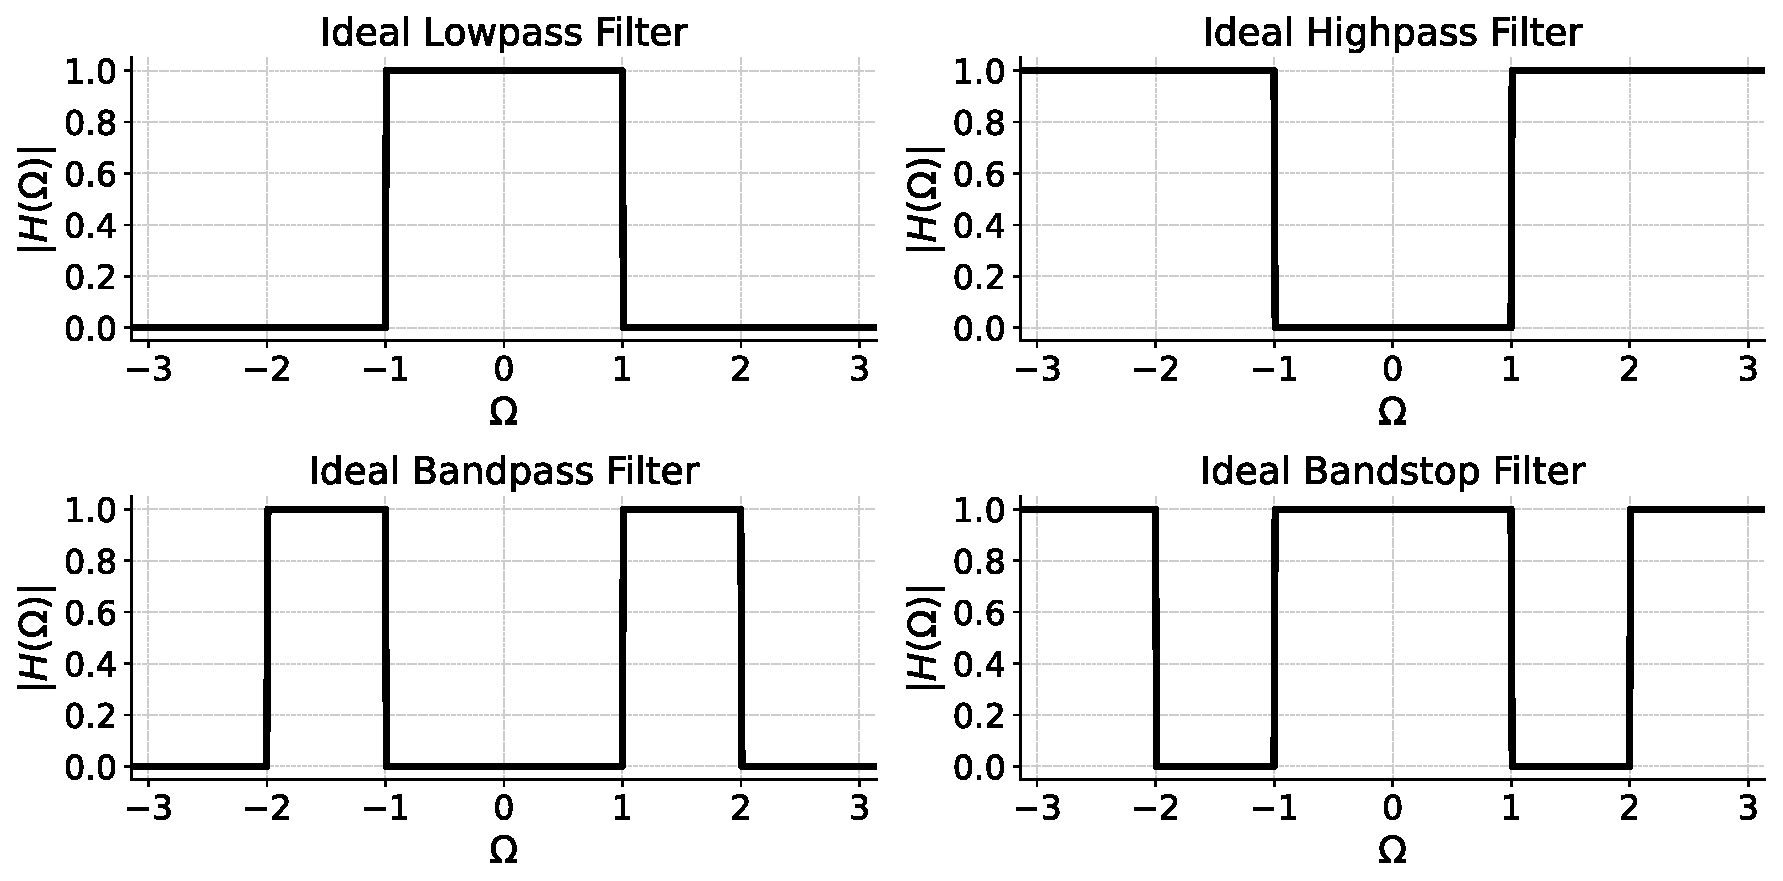
\includegraphics[width=0.9\textwidth]{img/idealfilt.eps}
%   \end{figure}
%   \end{center}
% \end{frame}

\end{document}